\PassOptionsToPackage{unicode=true}{hyperref} % options for packages loaded elsewhere
\PassOptionsToPackage{hyphens}{url}
%


\documentclass[]{article}

\usepackage{ctex}
\setCJKmainfont{SimSun}
\usepackage{xeCJK} % 中文支持
% \setCJKmainfont{Noto Serif CJK SC} % 设置中文字体为宋体
\usepackage{lmodern}
\usepackage{amssymb,amsmath}
\usepackage{ifxetex,ifluatex}
\usepackage{fixltx2e} % provides \textsubscript
\ifnum 0\ifxetex 1\fi\ifluatex 1\fi=0 % if pdftex
  \usepackage[T1]{fontenc}
  \usepackage[utf8]{inputenc}
  \usepackage{textcomp} % provides euro and other symbols
\else % if luatex or xelatex
  \usepackage{unicode-math}
  \defaultfontfeatures{Ligatures=TeX,Scale=MatchLowercase}
\fi
% use upquote if available, for straight quotes in verbatim environments
\IfFileExists{upquote.sty}{\usepackage{upquote}}{}
% use microtype if available
\IfFileExists{microtype.sty}{%
\usepackage[]{microtype}
\UseMicrotypeSet[protrusion]{basicmath} % disable protrusion for tt fonts
}{}
\IfFileExists{parskip.sty}{%
\usepackage{parskip}
}{% else
\setlength{\parindent}{0pt}
\setlength{\parskip}{6pt plus 2pt minus 1pt}
}
\usepackage{hyperref}
\hypersetup{
            pdfborder={0 0 0},
            breaklinks=true}
\urlstyle{same}  % don't use monospace font for urls
\usepackage{longtable,booktabs}
% Fix footnotes in tables (requires footnote package)
\IfFileExists{footnote.sty}{\usepackage{footnote}\makesavenoteenv{longtable}}{}
\usepackage{graphicx,grffile}
\makeatletter
\def\maxwidth{\ifdim\Gin@nat@width>\linewidth\linewidth\else\Gin@nat@width\fi}
\def\maxheight{\ifdim\Gin@nat@height>\textheight\textheight\else\Gin@nat@height\fi}
\makeatother
% Scale images if necessary, so that they will not overflow the page
% margins by default, and it is still possible to overwrite the defaults
% using explicit options in \includegraphics[width, height, ...]{}
\setkeys{Gin}{width=\maxwidth,height=\maxheight,keepaspectratio}
\setlength{\emergencystretch}{3em}  % prevent overfull lines
\providecommand{\tightlist}{%
  \setlength{\itemsep}{0pt}\setlength{\parskip}{0pt}}
\setcounter{secnumdepth}{0}
% Redefines (sub)paragraphs to behave more like sections
\ifx\paragraph\undefined\else
\let\oldparagraph\paragraph
\renewcommand{\paragraph}[1]{\oldparagraph{#1}\mbox{}}
\fi
\ifx\subparagraph\undefined\else
\let\oldsubparagraph\subparagraph
\renewcommand{\subparagraph}[1]{\oldsubparagraph{#1}\mbox{}}
\fi

% set default figure placement to htbp
\makeatletter
\def\fps@figure{htbp}
\makeatother


\date{}

\begin{document}

\begin{center}
  \protect\hypertarget{_Hlk208135206}{}{}\LARGE 商业综合体信息管理系统\\[6pt]
  \large 系统设计与实现文档\\[12pt]
  \normalsize
  2351454\quad 黄文\\
  2353935\quad 刘逸飞\\
  2251597\quad 韦瑾钰\\
  2353926\quad 赵泽远\\
  2351041\quad 刘浩田\\
  2351880\quad 郑淑涵\\
  2350284\quad 张俊峰\\
  2352736\quad 孙一宁\\
  2250832\quad 李杜若
\end{center}

\bigskip
目 录

\protect\hyperlink{_Toc77076512}{{1.} 商业综合体信息管理{系统需求} 1}

\protect\hyperlink{ux7cfbux7edfux529fux80fdux6027ux9700ux6c42}{1.1
  系统功能性需求 1}

\protect\hyperlink{ux7528ux6237ux767bux5f55ux529fux80fdux6570ux636eux9700ux6c42}{1.1.1
  用户登录功能数据需求 1}

\protect\hyperlink{ux7528ux6237ux6ce8ux518cux529fux80fdux6570ux636eux9700ux6c42}{1.1.2
  用户注册功能数据需求 1}

\protect\hyperlink{ux7528ux6237ux4fe1ux606fux7ba1ux7406ux529fux80fdux6570ux636eux9700ux6c42}{1.1.3
  用户信息管理功能数据需求 1}

\protect\hyperlink{ux533aux57dfux4fe1ux606fux7ba1ux7406ux529fux80fdux6570ux636eux9700ux6c42}{1.1.4
  区域信息管理功能数据需求 1}

\protect\hyperlink{ux5408ux4f5cux65b9ux4fe1ux606fux67e5ux8be2ux529fux80fdux6570ux636eux9700ux6c42}{1.1.5
  合作方信息查询功能数据需求 2}

\protect\hyperlink{ux5408ux4f5cux65b9ux4fe1ux606fux4feeux6539ux529fux80fdux6570ux636eux9700ux6c42}{1.1.6
  合作方信息修改功能数据需求 2}

\protect\hyperlink{ux5408ux4f5cux65b9ux7edfux8ba1ux4fe1ux606fux62a5ux8868ux6570ux636eux9700ux6c42}{1.1.7
  合作方统计信息报表数据需求 2}

\protect\hyperlink{ux573aux5730ux9884ux7ea6ux529fux80fdux6570ux636eux9700ux6c42}{1.1.8
  场地预约功能数据需求 2}

\protect\hyperlink{ux573aux5730ux6d3bux52a8ux7ba1ux7406ux529fux80fdux6570ux636eux9700ux6c42}{1.1.9
  场地活动管理功能数据需求 2}

\protect\hyperlink{ux573aux5730ux6d3bux52a8ux7ed3ux7b97ux6536ux8d39ux529fux80fdux6570ux636eux9700ux6c42}{1.1.10
  场地活动结算收费功能数据需求 2}

\protect\hyperlink{ux573aux5730ux6d3bux52a8ux7edfux8ba1ux6570ux636eux62a5ux8868ux751fux6210ux529fux80fd}{1.1.11
  场地活动统计数据报表生成功能 3}

\protect\hyperlink{ux4fc3ux9500ux6d3bux52a8ux7ba1ux7406ux529fux80fdux6570ux636eux9700ux6c42}{1.1.12
  促销活动管理功能数据需求 3}

\protect\hyperlink{ux4fc3ux9500ux6d3bux52a8ux7edfux8ba1ux6570ux636eux62a5ux8868ux751fux6210ux529fux80fd}{1.1.13
  促销活动统计数据报表生成功能 3}

\protect\hyperlink{ux5458ux5de5ux6743ux9650ux7ba1ux7406ux529fux80fdux6570ux636eux9700ux6c42}{1.1.14
  员工权限管理功能数据需求 3}

\protect\hyperlink{ux5458ux5de5ux4e2aux4ebaux4fe1ux606fux4feeux6539ux529fux80fdux6570ux636eux9700ux6c42}{1.1.15
  员工个人信息修改功能数据需求 3}

\protect\hyperlink{ux5458ux5de5ux8003ux52e4ux529fux80fdux6570ux636eux9700ux6c42}{1.1.16
  员工考勤功能数据需求 3}

\protect\hyperlink{ux5458ux5de5ux5de5ux8d44ux7ba1ux7406ux529fux80fdux6570ux636eux9700ux6c42}{1.1.17
  员工工资管理功能数据需求 4}

\protect\hyperlink{ux5458ux5de5ux5de5ux8d44ux7edfux8ba1ux62a5ux8868ux751fux6210ux529fux80fdux6570ux636eux9700ux6c42}{1.1.18
  员工工资统计报表生成功能数据需求 4}

\protect\hyperlink{ux5458ux5de5ux4e34ux65f6ux6743ux9650ux7ba1ux7406ux529fux80fdux6570ux636eux9700ux6c42}{1.1.19
  员工临时权限管理功能数据需求 4}

\protect\hyperlink{ux5546ux6237ux4fe1ux606fux7ba1ux7406ux529fux80fdux6570ux636eux9700ux6c42}{1.1.20
  商户信息管理功能数据需求 4}

\protect\hyperlink{ux5e97ux9762ux72b6ux6001ux7ba1ux7406ux529fux80fdux6570ux636eux9700ux6c42}{1.1.21
  店面状态管理功能数据需求 4}

\protect\hyperlink{ux5546ux6237ux4fe1ux606fux7edfux8ba1ux62a5ux8868ux529fux80fdux6570ux636eux9700ux6c42}{1.1.22
  商户信息统计报表功能数据需求 4}

\protect\hyperlink{ux5546ux6237ux79dfux91d1ux6536ux53d6ux529fux80fdux6570ux636eux9700ux6c42}{1.1.23
  商户租金收取功能数据需求 4}

\protect\hyperlink{ux5546ux6237ux79dfux91d1ux7edfux8ba1ux62a5ux8868ux529fux80fdux6570ux636eux9700ux6c42}{1.1.24
  商户租金统计报表功能数据需求 5}

\protect\hyperlink{ux505cux8f66ux573aux8f66ux4f4dux72b6ux6001ux67e5ux8be2ux529fux80fdux6570ux636eux9700ux6c42}{1.1.25
  停车场车位状态查询功能数据需求 5}

\protect\hyperlink{ux505cux8f66ux573aux51faux5165ux8f66ux8ba1ux8d39ux529fux80fdux6570ux636eux9700ux6c42}{1.1.26
  停车场出入车计费功能数据需求 5}

\protect\hyperlink{ux505cux8f66ux573aux7edfux8ba1ux4fe1ux606fux62a5ux8868ux529fux80fdux6570ux636eux9700ux6c42}{1.1.27
  停车场统计信息报表功能数据需求 5}

\protect\hyperlink{ux8bbeux5907ux76d1ux63a7ux548cux64cdux4f5cux529fux80fdux6570ux636eux9700ux6c42}{1.1.28
  设备监控和操作功能数据需求 5}

\protect\hyperlink{ux8bbeux5907ux7ef4ux62a4ux5de5ux5355ux529fux80fdux6570ux636eux9700ux6c42}{1.1.29
  设备维护工单功能数据需求 5}

\protect\hyperlink{ux7efcux5408ux73b0ux91d1ux6d41ux62a5ux8868ux529fux80fdux6570ux636eux9700ux6c42}{1.1.30
  综合现金流报表功能数据需求 5}

\protect\hyperlink{ux7cfbux7edfux975eux529fux80fdux6027ux9700ux6c42}{1.2
  系统非功能性需求 6}

\protect\hyperlink{ux6027ux80fdux9700ux6c42}{1.2.1 性能需求 6}

\protect\hyperlink{ux53efux9760ux6027ux9700ux6c42}{1.2.2 可靠性需求 6}

\protect\hyperlink{ux517cux5bb9ux6027ux9700ux6c42}{1.2.3 兼容性需求 6}

\protect\hyperlink{ux73afux5883ux9700ux6c42}{1.2.4 环境需求 6}

\protect\hyperlink{ux53efux9760ux6027ux9700ux6c42-1}{1.2.5 可靠性需求 6}

\protect\hyperlink{ux53efux6d4bux8bd5ux6027ux9700ux6c42}{1.2.6
  可测试性需求 6}

\protect\hyperlink{_Toc77076515}{{1.3} {组织结构} 1}

\protect\hyperlink{ux5546ux4e1aux7efcux5408ux4f53ux4fe1ux606fux7ba1ux7406ux7cfbux7edfux8bbeux8ba1ux4e0eux5b9eux73b0}{{2.}
商业综合体信息管理{系统设计与实现} 2}

\protect\hyperlink{ux7528ux6237ux7528ux4f8b}{{2.1} {**用例} 2}

\protect\hyperlink{ux7528ux6237ux7528ux4f8bux8bbeux8ba1}{{2.1.1}
    {**用例设计} 2}

\protect\hyperlink{ux7528ux6237ux7528ux4f8bux5b9eux73b0}{{2.1.2}
    {**用例实现} 2}

\protect\hyperlink{ux7528ux4f8b}{{2.2} {**用例} 3}

\protect\hyperlink{ux6570ux636eux5e93ux8bbeux8ba1}{{3.} {数据库设计} 4}

\protect\hyperlink{_Toc77076522}{{附录A.} {图表索引} 5}

\hypertarget{ux7cfbux7edfux9700ux6c42ux6982ux8ff0}{%
  \section{系统需求概述}\label{ux7cfbux7edfux9700ux6c42ux6982ux8ff0}}

本系统是为商业综合体管理人员设计的综合性信息管理平台,通过权限控制实现差异化数据访问和操作。系统涵盖区域管理、店铺管理、停车场管理、场地活动管理、设备管理、合作管理、员工权限管理、日志管理八大核心板块,支持业务流程闭环管理和数据分析功能。

\hypertarget{ux7cfbux7edfux529fux80fdux6027ux9700ux6c42}{%
  \subsection{系统功能性需求}\label{ux7cfbux7edfux529fux80fdux6027ux9700ux6c42}}

\hypertarget{ux7528ux6237ux767bux5f55ux529fux80fdux6570ux636eux9700ux6c42}{%
  \subsubsection{用户登录功能数据需求}\label{ux7528ux6237ux767bux5f55ux529fux80fdux6570ux636eux9700ux6c42}}

用户可以在首页进行登录。登录后则根据用户所属的权限分别跳转到员工界面/合作方界面/商户界面/管理员界面。在跳转后的页面可进行退出登录操作。

登录所需数据中用户名必须在3-10个字符之间,密码必须在6-15个字符之间,只能由ASCLL码表中可见字符组成,并且在数据库中加密存储。

\textbf{所需数据}:用户名、密码

\hypertarget{ux7528ux6237ux6ce8ux518cux529fux80fdux6570ux636eux9700ux6c42}{%
  \subsubsection{用户注册功能数据需求}\label{ux7528ux6237ux6ce8ux518cux529fux80fdux6570ux636eux9700ux6c42}}

用户可以在首页进行注册,注册可选员工/合作方/商户。注册后将到登录页面。

注册所需数据中用户名必须在3-10个字符之间且在数据库中没有重复,密码必须在6-15个字符之间,只能由ASCLL码表中可见字符组成,并且在数据库中加密存储。联系方式需要验证码验证。

第一个注册的用户会成为最高权限的管理员,并且可以指定其他新管理员,任何管理员可以修改其他非管理员用户的身份。

\textbf{所需数据}:用户名、密码、联系方式

\hypertarget{ux7528ux6237ux4fe1ux606fux7ba1ux7406ux529fux80fdux6570ux636eux9700ux6c42}{%
  \subsubsection{用户信息管理功能数据需求}\label{ux7528ux6237ux4fe1ux606fux7ba1ux7406ux529fux80fdux6570ux636eux9700ux6c42}}

用户可在登录后进入个人信息页面查看和修改个人信息,系统将根据用户身份限制可修改字段范围,修改后数据实时更新至数据库,用户可主动退出或保存后返回主界面。

\textbf{所需数据:}用户名、密码、联系方式、身份类型、所属部门、长期职位、可修改字段列表(如邮箱、电话、头像、紧急联系人)区域信息查询功能数据需求

\hypertarget{ux533aux57dfux4fe1ux606fux7ba1ux7406ux529fux80fdux6570ux636eux9700ux6c42}{%
  \subsubsection{区域信息管理功能数据需求}\label{ux533aux57dfux4fe1ux606fux7ba1ux7406ux529fux80fdux6570ux636eux9700ux6c42}}

拥有查询权限的管理人员可按区域ID、楼层、类型或空置状态检索区域信息,系统返回区域ID、是否空置、面积、类别、店面租金、场地费及当前租户或用途信息,查询结果支持列表与地图视图.

\textbf{所需数据}:账号权限、区域ID、楼层类型、空置状态

\hypertarget{ux5408ux4f5cux65b9ux4fe1ux606fux67e5ux8be2ux529fux80fdux6570ux636eux9700ux6c42}{%
  \subsubsection{合作方信息查询功能数据需求}\label{ux5408ux4f5cux65b9ux4fe1ux606fux67e5ux8be2ux529fux80fdux6570ux636eux9700ux6c42}}

权限达标的管理人员可查询合作方详细信息,包括联系方式和负责人信息。

合作对象ID为唯一标识符,联系方式需包含电话和邮箱。

\textbf{所需数据}:账号权限、合作对象ID、合作方名称、负责人姓名、联系方式

\hypertarget{ux5408ux4f5cux65b9ux4fe1ux606fux4feeux6539ux529fux80fdux6570ux636eux9700ux6c42}{%
  \subsubsection{合作方信息修改功能数据需求}\label{ux5408ux4f5cux65b9ux4fe1ux606fux4feeux6539ux529fux80fdux6570ux636eux9700ux6c42}}

项目经理可修改合作方信息及关联活动状态,需权限校验。

合作活动申请状态包括"审批中/进行中/已完成"三种状态。

\textbf{所需数据}:账号权限、合作对象ID、合作方名称、负责人姓名、联系方式、合作活动申请状态

\hypertarget{ux5408ux4f5cux65b9ux7edfux8ba1ux4fe1ux606fux62a5ux8868ux6570ux636eux9700ux6c42}{%
  \subsubsection{合作方统计信息报表数据需求}\label{ux5408ux4f5cux65b9ux7edfux8ba1ux4fe1ux606fux62a5ux8868ux6570ux636eux9700ux6c42}}

系统按月/季度/年生成合作方统计报表,包含合作方总数、活动次数、总投资金额、平均活动收益、活跃合作方排名,支持按时间段、行业类型筛选并以图表和表格形式导出.

\textbf{所需数据}:时间范围、合作方ID、活动ID、投资金额、活动收入、行业分类

\hypertarget{ux573aux5730ux9884ux7ea6ux529fux80fdux6570ux636eux9700ux6c42}{%
  \subsubsection{场地预约功能数据需求}\label{ux573aux5730ux9884ux7ea6ux529fux80fdux6570ux636eux9700ux6c42}}

项目经理填写活动场地预约申请,由权限达标的管理人员审批。

租用时间需满足"结束时间\textgreater{}起始时间"规则,活动区域ID需为有效编码。

\textbf{所需数据}:合作对象ID、活动区域ID、租用起始时间、租用结束时间、租用用途、合作方名称、员工职位

\hypertarget{ux573aux5730ux6d3bux52a8ux7ba1ux7406ux529fux80fdux6570ux636eux9700ux6c42}{%
  \subsubsection{场地活动管理功能数据需求}\label{ux573aux5730ux6d3bux52a8ux7ba1ux7406ux529fux80fdux6570ux636eux9700ux6c42}}

活动获批后生成活动记录,项目经理可更新活动名称、参与人数、内容描述、状态(筹备中/进行中/已结束),系统记录修改日志,支持批量导入参与人员。

\textbf{所需数据}:活动ID、活动名、活动人数、内容描述、活动状态、账号权限、临时权限ID

\hypertarget{ux573aux5730ux6d3bux52a8ux7ed3ux7b97ux6536ux8d39ux529fux80fdux6570ux636eux9700ux6c42}{%
  \subsubsection{场地活动结算收费功能数据需求}\label{ux573aux5730ux6d3bux52a8ux7ed3ux7b97ux6536ux8d39ux529fux80fdux6570ux636eux9700ux6c42}}

活动结束后系统根据实际使用时长、场地费标准及附加服务自动生成结算单,项目经理确认后生成应收款,支持在线支付与发票申请。

\textbf{所需数据}:活动ID、活动区域ID、租用起始时间、租用结束时间、场地费、附加服务费、支付方式、开票信息

\hypertarget{ux573aux5730ux6d3bux52a8ux7edfux8ba1ux6570ux636eux62a5ux8868ux751fux6210ux529fux80fd}{%
  \subsubsection{场地活动统计数据报表生成功能}\label{ux573aux5730ux6d3bux52a8ux7edfux8ba1ux6570ux636eux62a5ux8868ux751fux6210ux529fux80fdux6570ux636eux9700ux6c42}}

系统按日/周/月生成场地活动统计报表,包含活动场次、总租用时长、总收费、平均上座率、热门场地排行,可导出PDF/Excel。

\textbf{所需数据}:活动ID、活动区域ID、租用起始时间、租用结束时间、场地费、实际参与人数

\hypertarget{ux4fc3ux9500ux6d3bux52a8ux7ba1ux7406ux529fux80fdux6570ux636eux9700ux6c42}{%
  \subsubsection{促销活动管理功能数据需求}\label{ux4fc3ux9500ux6d3bux52a8ux7ba1ux7406ux529fux80fdux6570ux636eux9700ux6c42}}

管理员或商户可创建促销活动,填写活动名称、促销花费、目标店铺、开始结束时间、折扣或满减规则,系统自动推送至关联店铺。

\textbf{所需数据}:活动ID、活动名称、促销花费、店铺ID列表、活动开始时间、活动结束时间、促销规则描述

\hypertarget{ux4fc3ux9500ux6d3bux52a8ux7edfux8ba1ux6570ux636eux62a5ux8868ux751fux6210ux529fux80fd}{%
  \subsubsection{促销活动统计数据报表生成功能}\label{ux4fc3ux9500ux6d3bux52a8ux7edfux8ba1ux6570ux636eux62a5ux8868ux751fux6210ux529fux80fdux6570ux636eux9700ux6c42}}

系统在促销活动结束后生成效果报表,包括参与店铺数、总销售额增量、促销成本、ROI、优惠券核销率,支持按店铺或活动维度对比。

\textbf{所需数据}:活动ID、店铺ID、促销花费、销售额增量、优惠券使用量、时间范围

\hypertarget{ux5458ux5de5ux6743ux9650ux7ba1ux7406ux529fux80fdux6570ux636eux9700ux6c42}{%
  \subsubsection{员工权限管理功能数据需求}\label{ux5458ux5de5ux6743ux9650ux7ba1ux7406ux529fux80fdux6570ux636eux9700ux6c42}}

人事管理员可新增、修改或撤销员工权限,权限按角色模板分配,变更即时生效并记录审计日志,支持批量导入与权限有效期设置。

\textbf{所需数据}:员工ID、账号权限、角色模板、授权管理员账号、生效时间、失效时间、变更原因

\hypertarget{ux5458ux5de5ux4e2aux4ebaux4fe1ux606fux4feeux6539ux529fux80fdux6570ux636eux9700ux6c42}{%
  \subsubsection{员工个人信息修改功能数据需求}\label{ux5458ux5de5ux4e2aux4ebaux4fe1ux606fux4feeux6539ux529fux80fdux6570ux636eux9700ux6c42}}

员工可在权限允许范围内修改个人非敏感信息,系统根据身份类型开放不同字段,修改后同步更新员工表与账号表,并记录修改日志。

\textbf{所需数据}:员工ID、可修改字段列表(如联系方式、紧急联系人、头像链接)、变更内容、修改时间、操作账号

\hypertarget{ux5458ux5de5ux8003ux52e4ux529fux80fdux6570ux636eux9700ux6c42}{%
  \subsubsection{员工考勤功能数据需求}\label{ux5458ux5de5ux8003ux52e4ux529fux80fdux6570ux636eux9700ux6c42}}

系统每日自动记录员工签到签退时间,允许补录与异常申诉,月末生成考勤汇总。

\textbf{所需数据}:员工ID、签到时间、签退时间、考勤状态(正常/迟到/早退/缺勤)、补录原因、申诉说明

\hypertarget{ux5458ux5de5ux5de5ux8d44ux7ba1ux7406ux529fux80fdux6570ux636eux9700ux6c42}{%
  \subsubsection{员工工资管理功能数据需求}\label{ux5458ux5de5ux5de5ux8d44ux7ba1ux7406ux529fux80fdux6570ux636eux9700ux6c42}}

人事部门每月根据考勤、奖金、罚金计算工资,支持批量导入与个别调整,工资单生成后员工可在线查看与确认。

\textbf{所需数据}:员工ID、底薪、奖金、罚金、考勤次数、实际薪水、发放月份、确认状态

\hypertarget{ux5458ux5de5ux5de5ux8d44ux7edfux8ba1ux62a5ux8868ux751fux6210ux529fux80fdux6570ux636eux9700ux6c42}{%
  \subsubsection{员工工资统计报表生成功能数据需求}\label{ux5458ux5de5ux5de5ux8d44ux7edfux8ba1ux62a5ux8868ux751fux6210ux529fux80fdux6570ux636eux9700ux6c42}}

员工工资统计报表生成功能数据需求
系统按月生成工资总览报表,包含部门工资总额、人均工资、最高最低值、奖金罚金分布,支持导出与图表展示。

\textbf{所需数据}:时间(月份)、员工ID、部门、底薪、奖金、罚金、实际薪水

\hypertarget{ux5458ux5de5ux4e34ux65f6ux6743ux9650ux7ba1ux7406ux529fux80fdux6570ux636eux9700ux6c42}{%
  \subsubsection{员工临时权限管理功能数据需求}\label{ux5458ux5de5ux4e34ux65f6ux6743ux9650ux7ba1ux7406ux529fux80fdux6570ux636eux9700ux6c42}}

项目经理可为活动临时授权员工,权限在活动结束后自动回收,系统记录授权与回收日志。

\textbf{所需数据}:授权人账号、员工ID、活动ID、临时权限内容、授权时间、回收时间、活动结束标记

\hypertarget{ux5546ux6237ux4fe1ux606fux7ba1ux7406ux529fux80fdux6570ux636eux9700ux6c42}{%
  \subsubsection{商户信息管理功能数据需求}\label{ux5546ux6237ux4fe1ux606fux7ba1ux7406ux529fux80fdux6570ux636eux9700ux6c42}}

管理人员可查看与更新店铺及租户信息,支持按店铺ID、租户名称、状态检索,修改后同步更新店铺表。

\textbf{所需数据}:店铺ID、店铺名称、店铺状态、租户类型、租户名、租户联系方式、租用起始时间、租用结束时间、租金提交状态

\hypertarget{ux5e97ux9762ux72b6ux6001ux7ba1ux7406ux529fux80fdux6570ux636eux9700ux6c42}{%
  \subsubsection{店面状态管理功能数据需求}\label{ux5e97ux9762ux72b6ux6001ux7ba1ux7406ux529fux80fdux6570ux636eux9700ux6c42}}

区域管理员可变更店面空置状态,更新租金或面积,变更前校验是否存在有效租约,所有变更记录入日志。

\textbf{所需数据}:区域ID、空置标识、面积、店铺租金、变更原因、操作账号

\hypertarget{ux5546ux6237ux4fe1ux606fux7edfux8ba1ux62a5ux8868ux529fux80fdux6570ux636eux9700ux6c42}{%
  \subsubsection{商户信息统计报表功能数据需求}\label{ux5546ux6237ux4fe1ux606fux7edfux8ba1ux62a5ux8868ux529fux80fdux6570ux636eux9700ux6c42}}

商户信息统计报表功能数据需求
系统实时生成商户运营报表,包含总店铺数、正常营业/空置/停业比例、租户行业分布、租金收缴率,可导出为PDF。

\textbf{所需数据}:店铺ID、店铺状态、租户类型、租用起始时间、租用结束时间、租金提交状态

\hypertarget{ux5546ux6237ux79dfux91d1ux6536ux53d6ux529fux80fdux6570ux636eux9700ux6c42}{%
  \subsubsection{商户租金收取功能数据需求}\label{ux5546ux6237ux79dfux91d1ux6536ux53d6ux529fux80fdux6570ux636eux9700ux6c42}}

租户登录店铺账号后查看应付租金并在线支付,系统生成电子收据并更新租金提交状态,逾期自动提醒。

\textbf{所需数据}:店铺ID、租户账号、应付金额、支付时间、支付方式、支付状态、收据编号

\hypertarget{ux5546ux6237ux79dfux91d1ux7edfux8ba1ux62a5ux8868ux529fux80fdux6570ux636eux9700ux6c42}{%
  \subsubsection{商户租金统计报表功能数据需求}\label{ux5546ux6237ux79dfux91d1ux7edfux8ba1ux62a5ux8868ux529fux80fdux6570ux636eux9700ux6c42}}

商户租金统计报表功能数据需求
系统按周期生成租金收入报表,展示应收、实收、欠费、逾期天数、收缴率及趋势图。

\textbf{所需数据}:店铺ID、区域ID、店面租金、租用起始时间、租用结束时间、租金提交状态、支付时间

\hypertarget{ux505cux8f66ux573aux8f66ux4f4dux72b6ux6001ux67e5ux8be2ux529fux80fdux6570ux636eux9700ux6c42}{%
  \subsubsection{停车场车位状态查询功能数据需求}\label{ux505cux8f66ux573aux8f66ux4f4dux72b6ux6001ux67e5ux8be2ux529fux80fdux6570ux636eux9700ux6c42}}

系统实时展示各停车场区域的车位占用情况,支持按区域、楼层、车位ID筛选,并提供剩余车位数统计。

\textbf{所需数据}:区域ID、车位ID、是否有车、更新时间、查询账号权限

\hypertarget{ux505cux8f66ux573aux51faux5165ux8f66ux8ba1ux8d39ux529fux80fdux6570ux636eux9700ux6c42}{%
  \subsubsection{停车场出入车计费功能数据需求}\label{ux505cux8f66ux573aux51faux5165ux8f66ux8ba1ux8d39ux529fux80fdux6570ux636eux9700ux6c42}}

车辆入场时自动抓拍车牌并分配车位,出场时按停车时长计费,支持现金、扫码、无感支付,系统记录完整流水。

\textbf{所需数据}:车牌号、区域ID、车位ID、停车起始时间、停车结束时间、单位时间停车费、支付状态

\hypertarget{ux505cux8f66ux573aux7edfux8ba1ux4fe1ux606fux62a5ux8868ux529fux80fdux6570ux636eux9700ux6c42}{%
  \subsubsection{停车场统计信息报表功能数据需求}\label{ux505cux8f66ux573aux7edfux8ba1ux4fe1ux606fux62a5ux8868ux529fux80fdux6570ux636eux9700ux6c42}}

系统按日/周/月生成停车场运营报表,包含车流量、收入总额、平均停车时长、高峰时段车位利用率,支持图表与Excel导出。

\textbf{所需数据}:区域ID、车牌号、停车起始时间、停车结束时间、单位时间停车费

\hypertarget{ux8bbeux5907ux76d1ux63a7ux548cux64cdux4f5cux529fux80fdux6570ux636eux9700ux6c42}{%
  \subsubsection{设备监控和操作功能数据需求}\label{ux8bbeux5907ux76d1ux63a7ux548cux64cdux4f5cux529fux80fdux6570ux636eux9700ux6c42}}

管理员可实时查看设备运行状态并进行远程控制,系统记录操作日志与状态变更,异常自动报警。

\textbf{所需数据}:设备ID、类别、状态、接口、区域ID、操作指令、操作账号、操作时间

\hypertarget{ux8bbeux5907ux7ef4ux62a4ux5de5ux5355ux529fux80fdux6570ux636eux9700ux6c42}{%
  \subsubsection{设备维护工单功能数据需求}\label{ux8bbeux5907ux7ef4ux62a4ux5de5ux5355ux529fux80fdux6570ux636eux9700ux6c42}}

报修人提交工单后系统分配维修员工,维修完成后填写结果与花费,所有流程状态可追踪。

\textbf{所需数据}:设备ID、员工ID、维修开始时间、维修结束时间、维修花费、故障描述、处理结果、工单状态

\hypertarget{ux7efcux5408ux73b0ux91d1ux6d41ux62a5ux8868ux529fux80fdux6570ux636eux9700ux6c42}{%
  \subsubsection{综合现金流报表功能数据需求}\label{ux7efcux5408ux73b0ux91d1ux6d41ux62a5ux8868ux529fux80fdux6570ux636eux9700ux6c42}}

综合现金流报表功能数据需求
系统每日自动汇总租金、停车费、活动收入、工资、维修、设备采购等现金收支,生成日报、月报、年报,支持按类别与时间段筛选。

\textbf{所需数据}:收入类型、支出类型、金额、发生时间、关联单据编号、账户余额

\hypertarget{ux7cfbux7edfux975eux529fux80fdux6027ux9700ux6c42}{%
  \subsection{系统非功能性需求}\label{ux7cfbux7edfux975eux529fux80fdux6027ux9700ux6c42}}

\hypertarget{ux6027ux80fdux9700ux6c42}{%
  \subsubsection{性能需求}\label{ux6027ux80fdux9700ux6c42}}

系统支持高效的数据查询与事务处理,可以确保在并发场景下稳定运行;后端部署于Ubuntu
22.04服务器,采用ASP.NET Core框架,前端基于Vue框架开发。

\textbf{所需数据}:操作系统,后端日志、前端框架、数据库、API 协议。

\hypertarget{ux53efux9760ux6027ux9700ux6c42}{%
  \subsubsection{可靠性需求}\label{ux53efux9760ux6027ux9700ux6c42}}

系统需具备高可用性,确保在长时间运行过程中稳定可靠。系统支持持续运行,减少计划外停机时间。

\textbf{所需数据}:系统可用性百分比、计划内维护时间、故障恢复时间(RTO)、数据恢复点(RPO)

\hypertarget{ux517cux5bb9ux6027ux9700ux6c42}{%
  \subsubsection{兼容性需求}\label{ux517cux5bb9ux6027ux9700ux6c42}}

系统需具备良好的兼容性,确保在不同环境下稳定运行。系统支持主流的浏览器和操作系统版本,确保前后端框架的兼容性。

\textbf{所需数据}:操作系统版本(Ubuntu 22.04)、后端框架版本(ASP.NET
Core)、前端框架版本(Vue)

\hypertarget{ux73afux5883ux9700ux6c42}{%
  \subsubsection{环境需求}\label{ux73afux5883ux9700ux6c42}}

系统运行环境基于 Ubuntu 22.04 操作系统,后端采用 ASP.NET Core
框架,前端使用 Vue 框架进行开发

\textbf{所需数据}:操作系统版本(Ubuntu 22.04)、后端框架版本(ASP.NET
Core)、前端框架版本(Vue)

\hypertarget{ux53efux9760ux6027ux9700ux6c42-1}{%
  \subsubsection{可靠性需求}\label{ux53efux9760ux6027ux9700ux6c42-1}}

系统需具备良好的可维护性,确保代码清晰、易于管理和更新。后端采用 ASP.NET
Core 框架,前端使用 Vue 框架,便于后续开发和维护

\textbf{所需数据}:代码规范、注释覆盖率、配置中心接口

\hypertarget{ux53efux6d4bux8bd5ux6027ux9700ux6c42}{%
  \subsubsection{可测试性需求}\label{ux53efux6d4bux8bd5ux6027ux9700ux6c42}}

系统需具备良好的可测试性,确保各功能模块能够进行有效的单元测试和集成测试。数据库设计中涉及的各个表和关系模式应支持独立测试,确保数据交互的准确性和完整性。同时,系统应支持对数据库操作的自动化测试,以验证数据的正确性和一致性

\textbf{所需数据}:单元测试覆盖率、接口自动化测试用例数、数据库操作测试覆盖率

\hypertarget{ux53efux7ef4ux62a4ux6027ux9700ux6c42}{%
  \subsubsection{可维护性需求}\label{ux53efux7ef4ux62a4ux6027ux9700ux6c42}}

系统需具备良好的可维护性,确保代码清晰、易于管理和更新。数据库设计应遵循规范化原则,确保数据结构合理,便于后续的扩展和维护。同时,系统应支持在线热更新配置,减少维护时间对业务的影响。

\textbf{所需数据}:数据库表结构设计文档、代码注释覆盖率、配置中心接口

\hypertarget{ux7ec4ux7ec7ux7ed3ux6784}{%
  \subsection{组织结构}\label{ux7ec4ux7ec7ux7ed3ux6784}}

列出文档的组织结构。

第一章:系统需求概述。展示我们设计的商业综合体信息管理系统的各功能对应的数据需求。

第二章:系统设计与实现。分析各系统功能的详细设计与代码实现。

第三章:数据库实现。分析数据库的具体实现。

附录A:是本文档的图表索引

\hypertarget{ux5546ux4e1aux7efcux5408ux4f53ux4fe1ux606fux7ba1ux7406ux7cfbux7edfux8bbeux8ba1ux4e0eux5b9eux73b0}{%
  \section{商业综合体信息管理系统设计与实现}\label{ux5546ux4e1aux7efcux5408ux4f53ux4fe1ux606fux7ba1ux7406ux7cfbux7edfux8bbeux8ba1ux4e0eux5b9eux73b0}}

本系统的使用者分为三类角色:管理员作为最高权限管理者,可全面掌控用户注册、区域划分、合作方审批、员工权限分配及现金流报表等核心功能;员工依据部门和职位权限,管理个人信息、考勤工资、活动申请及设备运维;商户则专注于自身店铺的运营,包括信息维护、租金缴纳、店面状态更新及促销活动参与。所有权限通过账号身份严格隔离。

\hypertarget{ux7528ux6237ux7528ux4f8b}{%
  \subsection{ 用户用例}\label{ux7528ux6237ux7528ux4f8b}}

\hypertarget{ux7528ux6237ux7528ux4f8bux8bbeux8ba1}{%
  \subsubsection{用户用例设计}\label{ux7528ux6237ux7528ux4f8bux8bbeux8ba1}}

\protect\hypertarget{_Toc153186375}{}{\protect\hypertarget{_Toc394245026}{}{}}表格
2‑1 用户功能的动作序列

\begin{longtable}[]{@{}ll@{}}
  \toprule
  动作序列 & 描述\tabularnewline
  \midrule
  \endhead
  登录   & 不同用户登录进入到不同页面。\tabularnewline
  注册   &
  访客在系统首页选择注册,填写必要信息后提交,系统校验并创建账号\tabularnewline
  修改信息 &
  用户进入``个人信息''页面,对可编辑字段进行修改并提交,系统校验后更新数据库\tabularnewline
  \bottomrule
\end{longtable}

用户登录活动图:

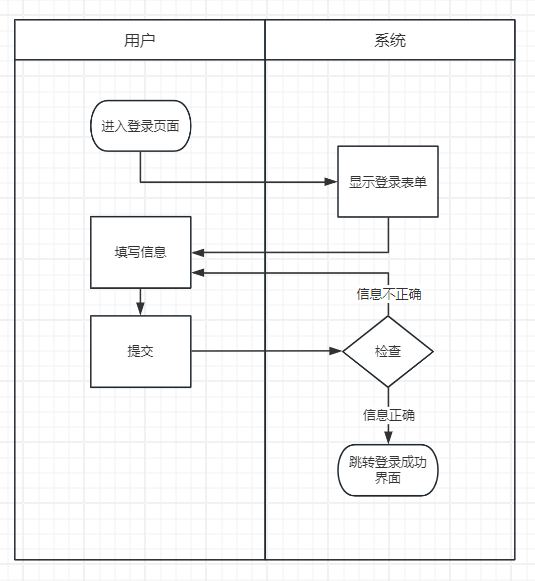
\includegraphics[width=4.45694in,height=4.83819in]{media/media/image1.png}

用户注册活动图:

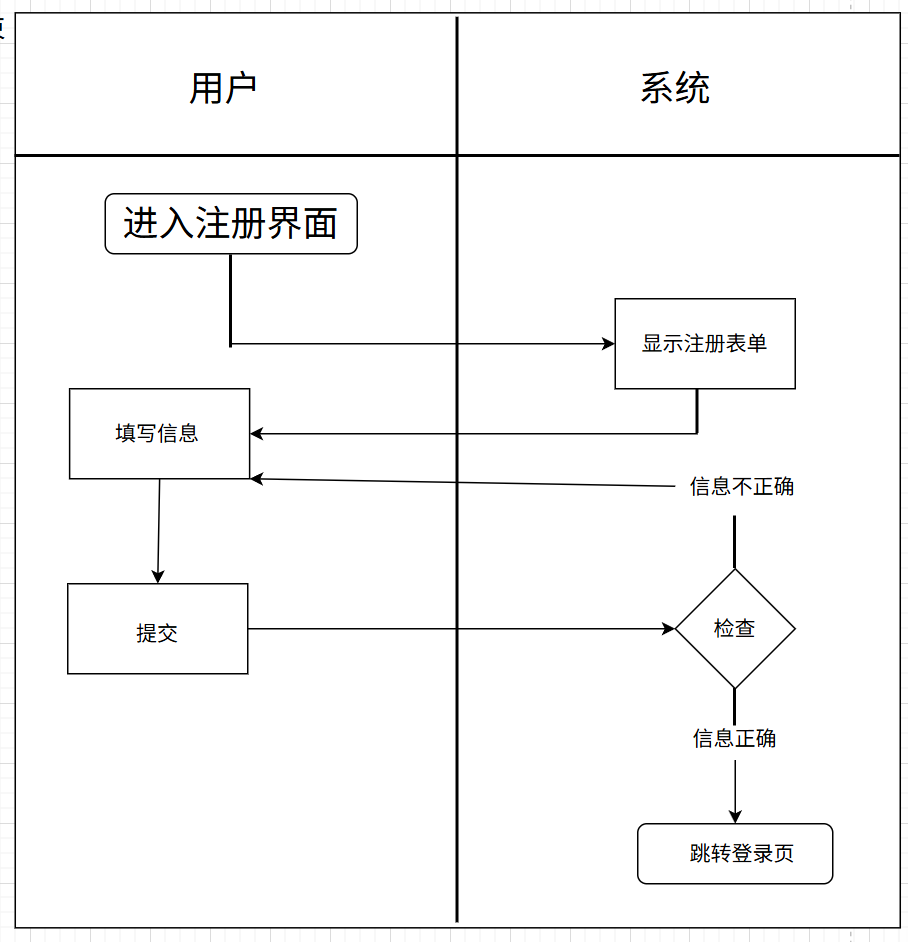
\includegraphics[width=4.35278in,height=4.51458in]{media/media/image2.png}

用户修改信息活动图:

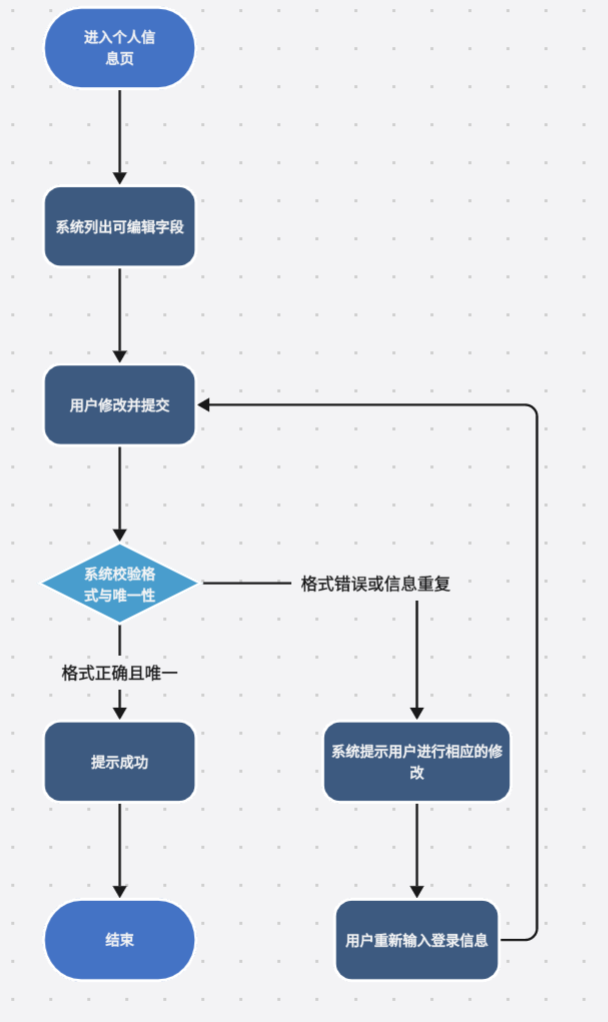
\includegraphics[width=2.82083in,height=4.73958in]{media/media/image3.png}

\hypertarget{ux7528ux6237ux7528ux4f8bux5b9eux73b0}{%
  \subsubsection{用户用例实现}\label{ux7528ux6237ux7528ux4f8bux5b9eux73b0}}

1. 主要类及其关系:

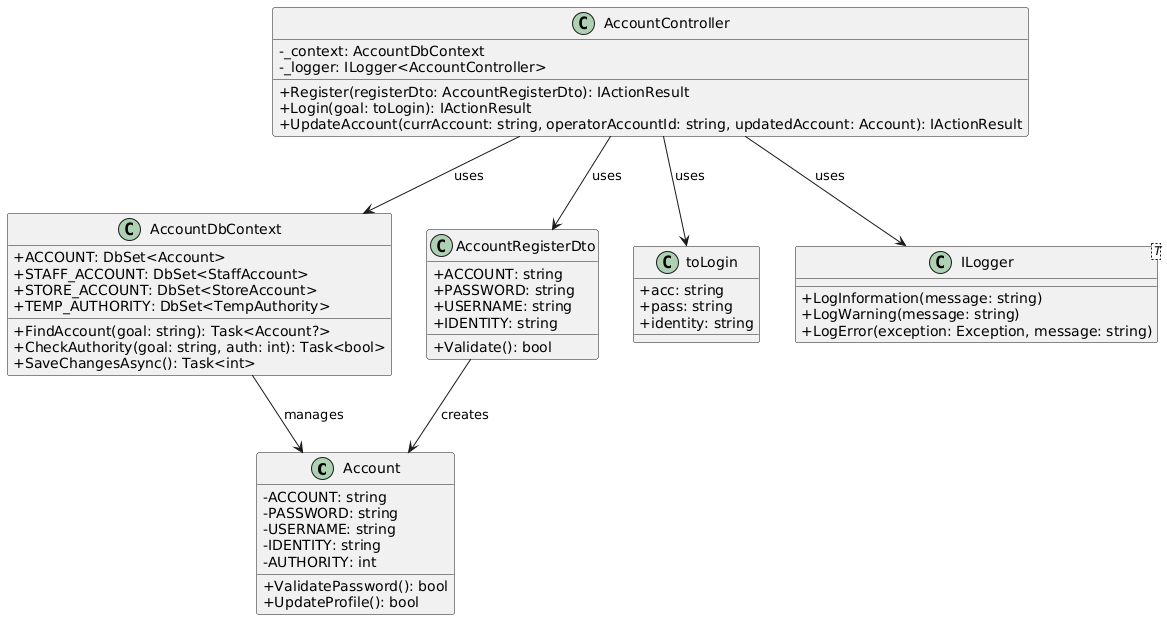
\includegraphics[width=6.06528in,height=3.22222in]{media/media/image4.png}

2. 方法设计与实现

用户登录:

~ ~ ~ ~ public class toLogin

~ ~ ~ ~ \{

~ ~ ~ ~ ~ ~ public string acc \{ get; set; \}

~ ~ ~ ~ ~ ~ public string pass \{ get; set; \}

~ ~ ~ ~ ~ ~ public string identity \{ get; set; \}

~ ~ ~ ~ \}

{[}HttpPost("login"){]}

~ ~ ~ ~ public async Task\textless{}IActionResult\textgreater{}
Login({[}FromBody{]} toLogin goal)

验证用户身份并授权访问系统。该方法接收登录凭证后,首先查询数据库验证账号是否存在,随后校验密码是否匹配,最后核查账户状态是否可用(未被封禁)以及身份标识是否正确。全部验证通过后,返回该账户的完整信息以建立用户会话。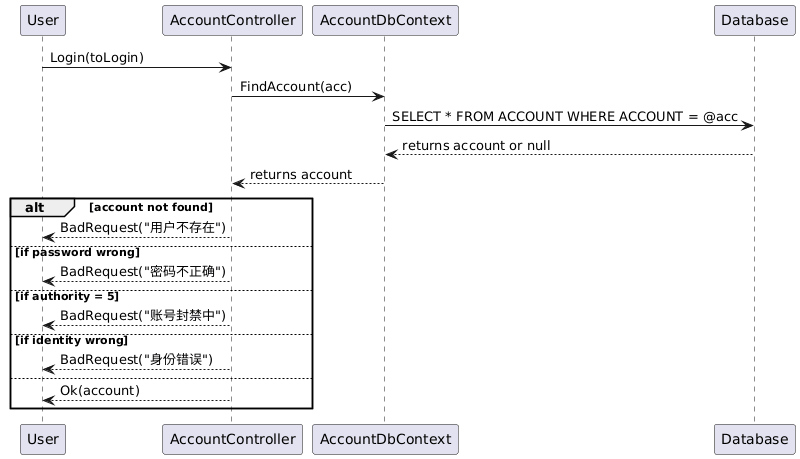
\includegraphics[width=5.88681in,height=3.37778in]{media/media/image5.png}

用户注册

在系统中创建新的用户账户。该方法会首先确保请求账号名的唯一性。对于系统首个注册的用户,将自动授予其最高管理员权限。后续注册则根据其选择的身份(``员工''或``商户'')分配相应的基础权限。最终,将新账户信息持久化至数据库,完成注册流程。

~ ~ ~ ~ public class AccountRegisterDto\{

~ ~ ~ ~ ~ ~ {[}Required(ErrorMessage = "账号为必填项"){]}

~ ~ ~ ~ ~ ~ {[}StringLength(50, MinimumLength = 3, ErrorMessage =
"账号长度必须在3到50个字符之间"){]}

~ ~ ~ ~ ~ ~ public string ACCOUNT \{ get; set; \}

~ ~ ~ ~ ~ ~ {[}Required(ErrorMessage = "密码为必填项"){]}

~ ~ ~ ~ ~ ~ {[}StringLength(100, MinimumLength = 6, ErrorMessage =
"密码长度至少为6个字符"){]}

~ ~ ~ ~ ~ ~ public string PASSWORD \{ get; set; \}

~ ~ ~ ~ ~ ~ {[}Required(ErrorMessage = "用户名为必填项"){]}

~ ~ ~ ~ ~ ~ {[}StringLength(50){]}

~ ~ ~ ~ ~ ~ public string USERNAME \{ get; set; \}

~ ~ ~ ~ ~ ~ {[}Required(ErrorMessage = "必须指定用户身份"){]}

~ ~ ~ ~ ~ ~ {[}StringLength(50){]}

~ ~ ~ ~ ~ ~ public string IDENTITY \{ get; set; \}

~ ~ ~ ~ \}

~ ~ ~ ~ {[}HttpPost("register"){]}

~ ~ ~ ~ public async Task\textless{}IActionResult\textgreater{}
Register({[}FromBody{]} AccountRegisterDto registerDto)

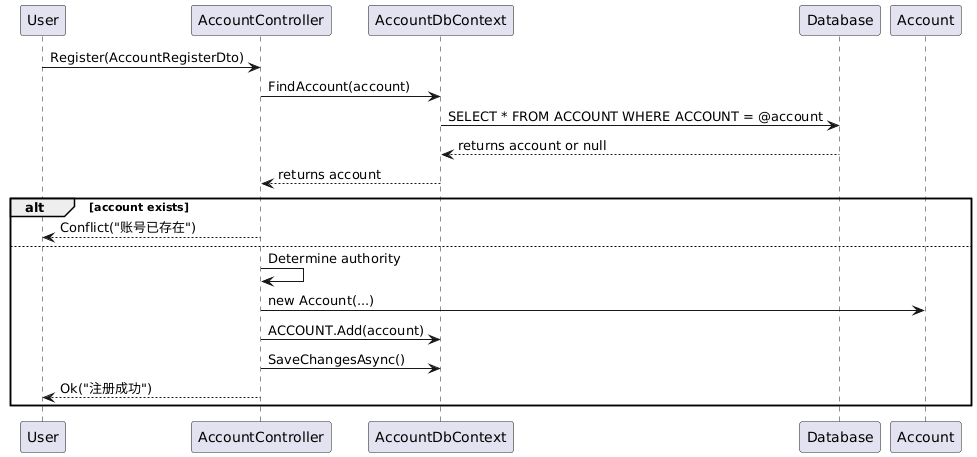
\includegraphics[width=5.75347in,height=2.69097in]{media/media/image6.png}

用户信息修改:

更新指定账户的详细信息。此操作需要由另一名已登录的操作员发起,并包含严格的权限校验逻辑以确保数据安全。仅允许系统管理员修改他人账户,且操作员的权限等级必须高于或等于其要修改的目标权限。该方法会防止关键字段(如账号名)被误修改,并确保身份等数据的有效性,最终将合规的变更安全地更新至数据库。

~ ~ ~ ~ {[}HttpPatch("alter/\{currAccount\}"){]}

~ ~ ~ ~ public async Task\textless{}IActionResult\textgreater{}
UpdateAccount(

~ ~ ~ ~ ~ ~ string currAccount,

~ ~ ~ ~ ~ ~ {[}FromQuery{]} string operatorAccountId,

~ ~ ~ ~ ~ ~ {[}FromBody{]} Account updatedAccount)

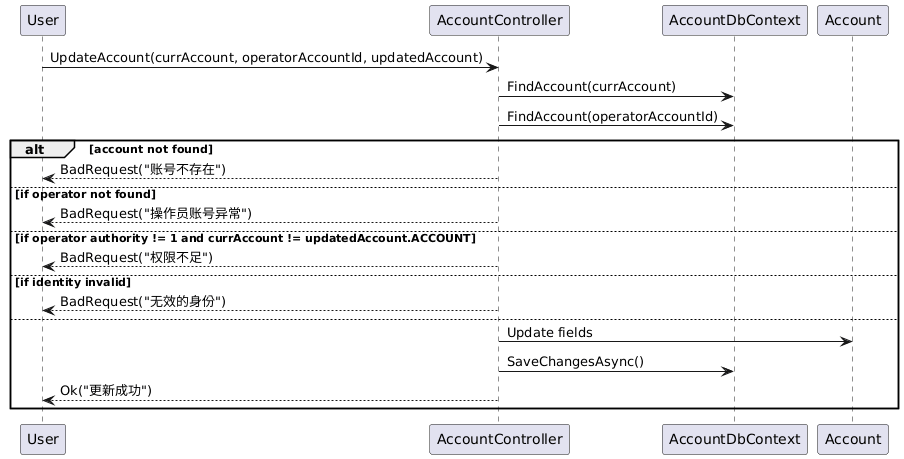
\includegraphics[width=5.64167in,height=2.86458in]{media/media/image7.png}

\hypertarget{ux7528ux4f8b}{%
  \subsection{**用例}\label{ux7528ux4f8b}}

依此类推。

\hypertarget{ux7528ux4f8b-1}{%
  \subsection{区域用例}\label{ux7528ux4f8b-1}}
\hypertarget{ux7528ux4f8b-1ux8bbeux8ba1}{%
  \subsubsection{区域用例设计}\label{ux7528ux4f8b-1ux8bbeux8ba1}}

% 区域用例设计表格

\begin{longtable}[]{@{}ll@{}}
  \toprule
  \textbf{动作序列} & \textbf{描述}                \\
  \midrule
  \endhead
  添加新区域         & 管理员在系统内新增一块可租用的区域,并设定其基础属性 \\
  区域信息查询        & 用户按条件检索区域列表并查看详情           \\
  区域信息管理        & 管理员对已有区域的基础属性进行修改或删除       \\
  \bottomrule
\end{longtable}

添加新区域活动图:

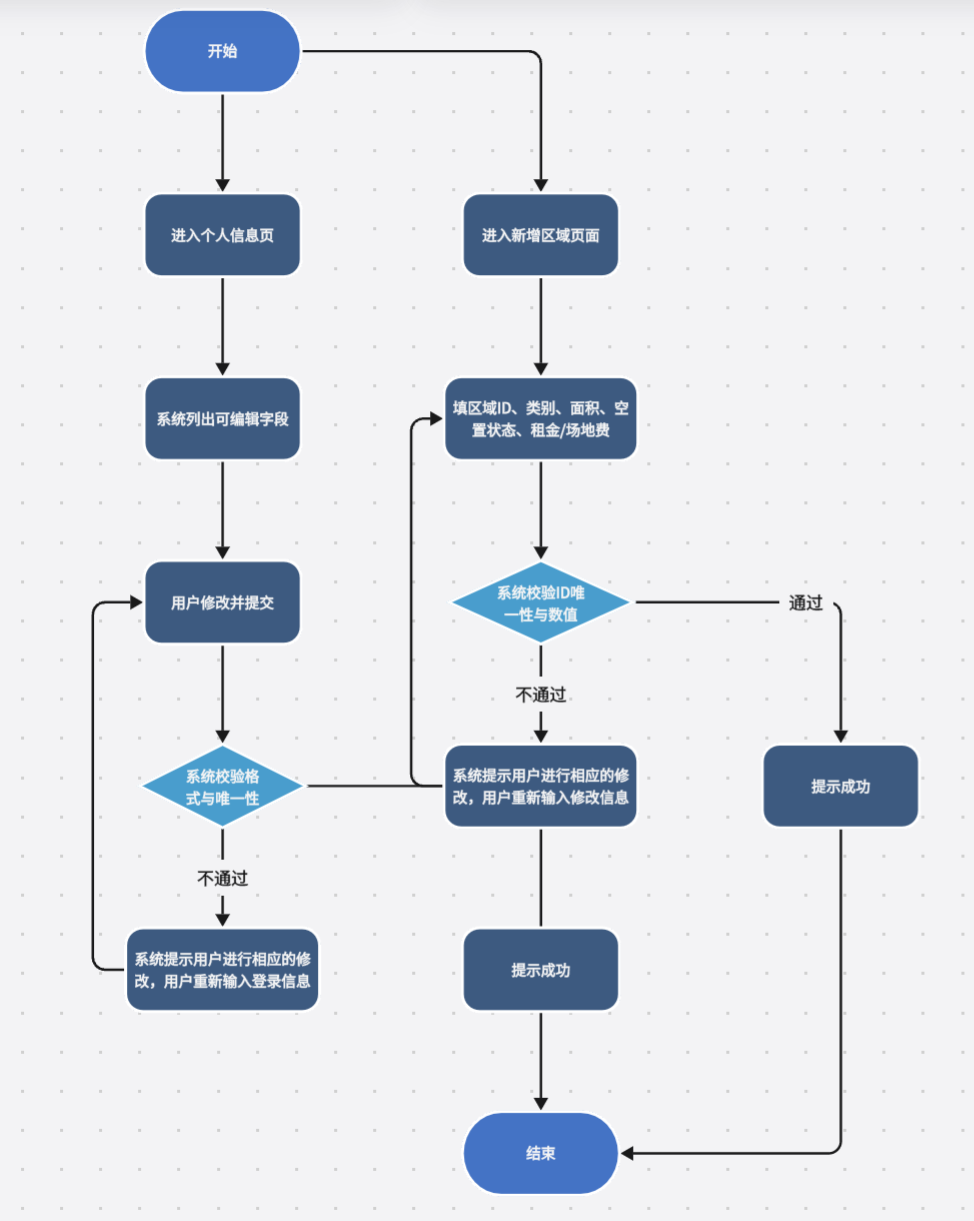
\includegraphics[width=4.45694in,height=4.83819in]{media/media/image_2-3-1.png}

区域信息查询活动图:

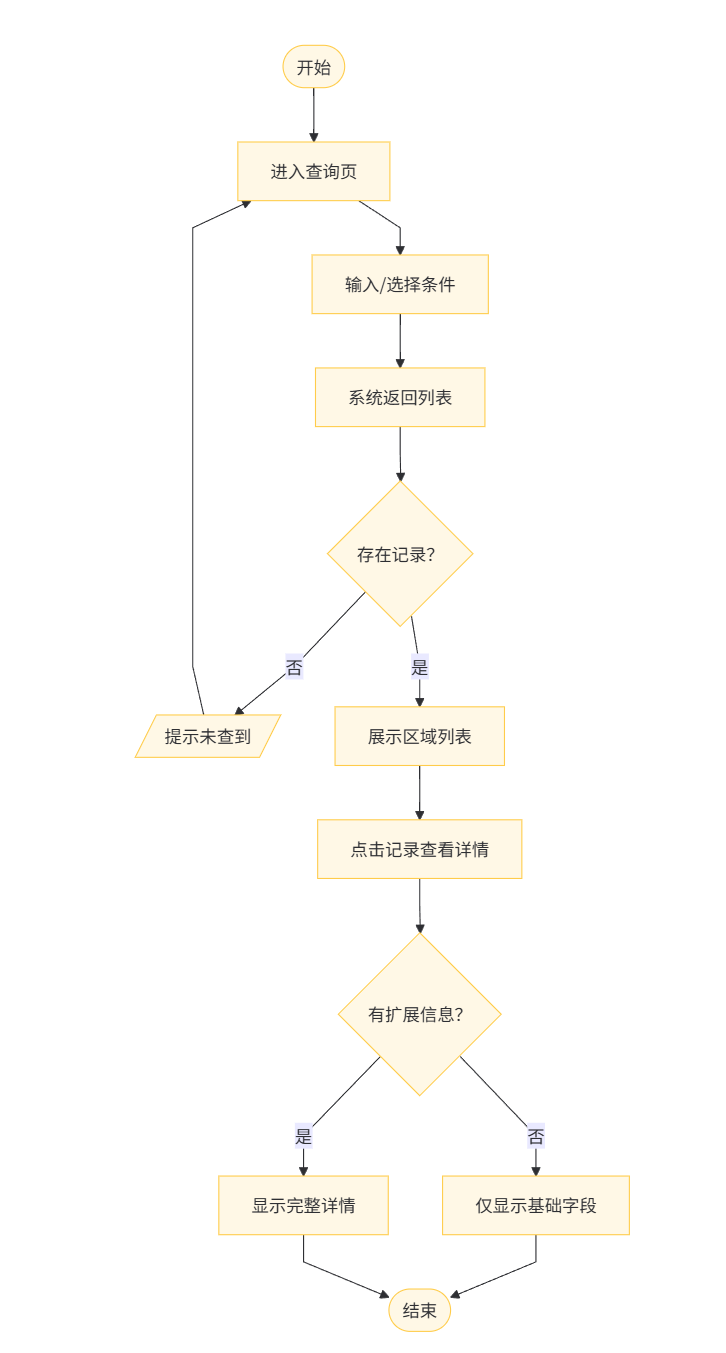
\includegraphics[width=4.45694in,height=4.83819in]{media/media/image_2-3-2.png}

区域信息管理活动图:

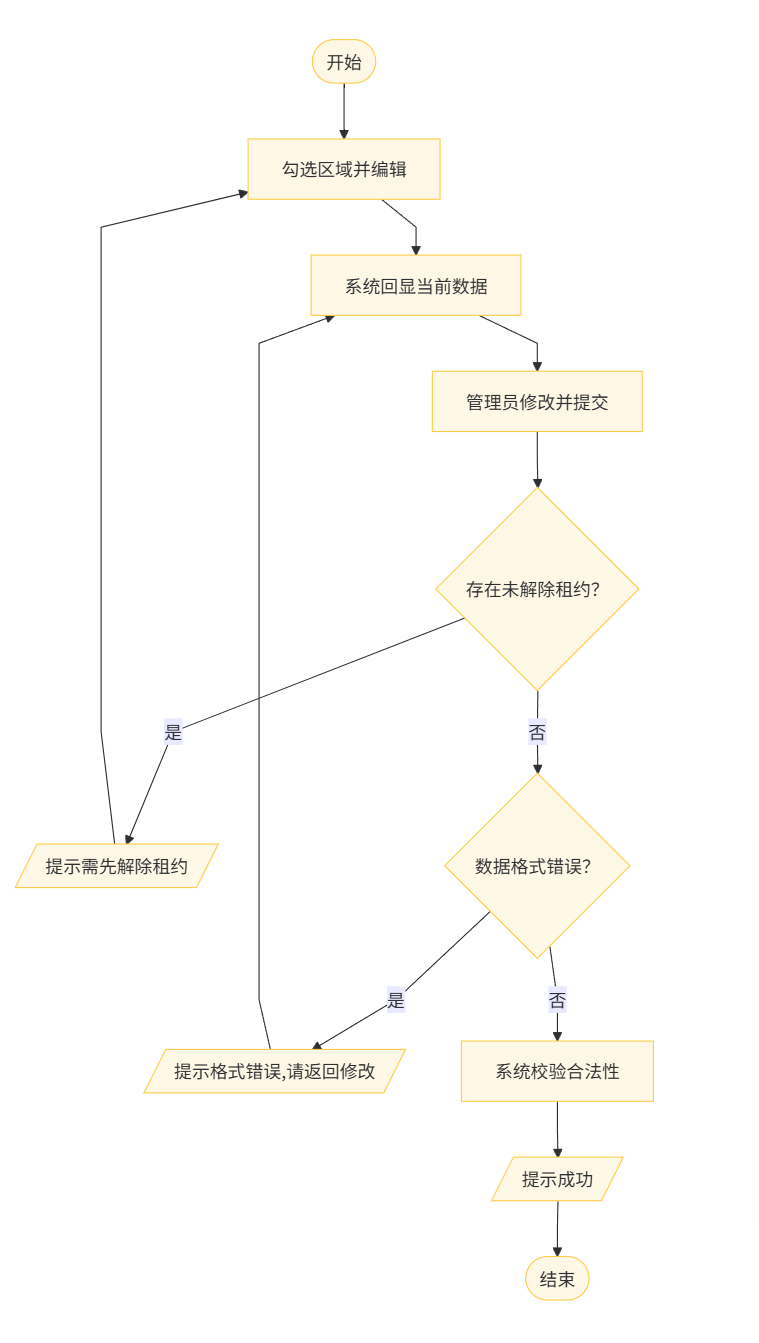
\includegraphics[width=4.45694in,height=4.83819in]{media/media/image_2-3-3.png}

\hypertarget{ux7528ux4f8b-1ux5b9eux73b0}{%
  \subsubsection{区域用例实现}\label{ux7528ux4f8b-1ux5b9eux73b0}}
1. 主要类及其关系:
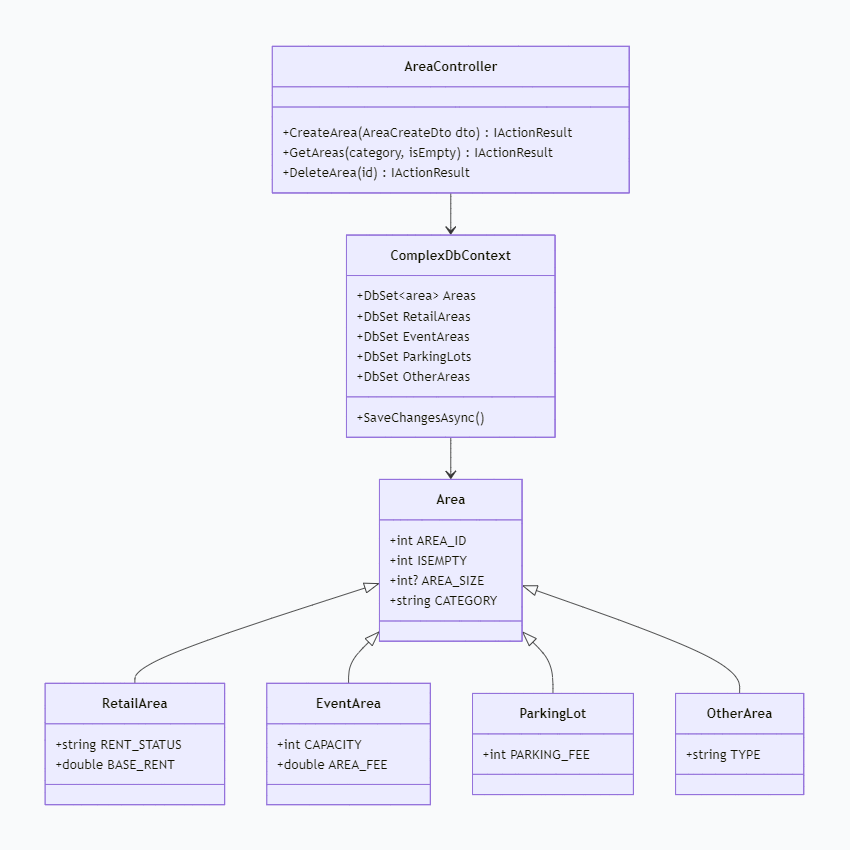
\includegraphics[width=6.06528in,height=3.22222in]{media/media/image_2-3-4.png}

2. 方法设计与实现

添加新区域

\begin{verbatim}
public class AreaCreateDto {
    public int AreaId { get; set; }
    public int IsEmpty { get; set; }
    public int? AreaSize { get; set; }
    [Required]
    public string Category { get; set; } // "RETAIL", "EVENT"
    // Retail-specific properties
    public string? RentStatus { get; set; }
    public double? BaseRent { get; set; }
    // Event-specific properties
    public int? Capacity { get; set; }
    public int? AreaFee { get; set; }
    // 其它类型
    public string? Type { get; set; }
    public int? ParkingFee { get; set; }
}
\end{verbatim}

\begin{verbatim}
[HttpPost]
public async Task<IActionResult> CreateArea([FromBody] AreaCreateDto dto)
\end{verbatim}
管理员通过传入 AreaCreateDto 对象创建新区域。系统会检查区域ID是否重复,并根据区域类别(RETAIL/EVENT/PARKING/OTHER)创建不同类型的区域记录。

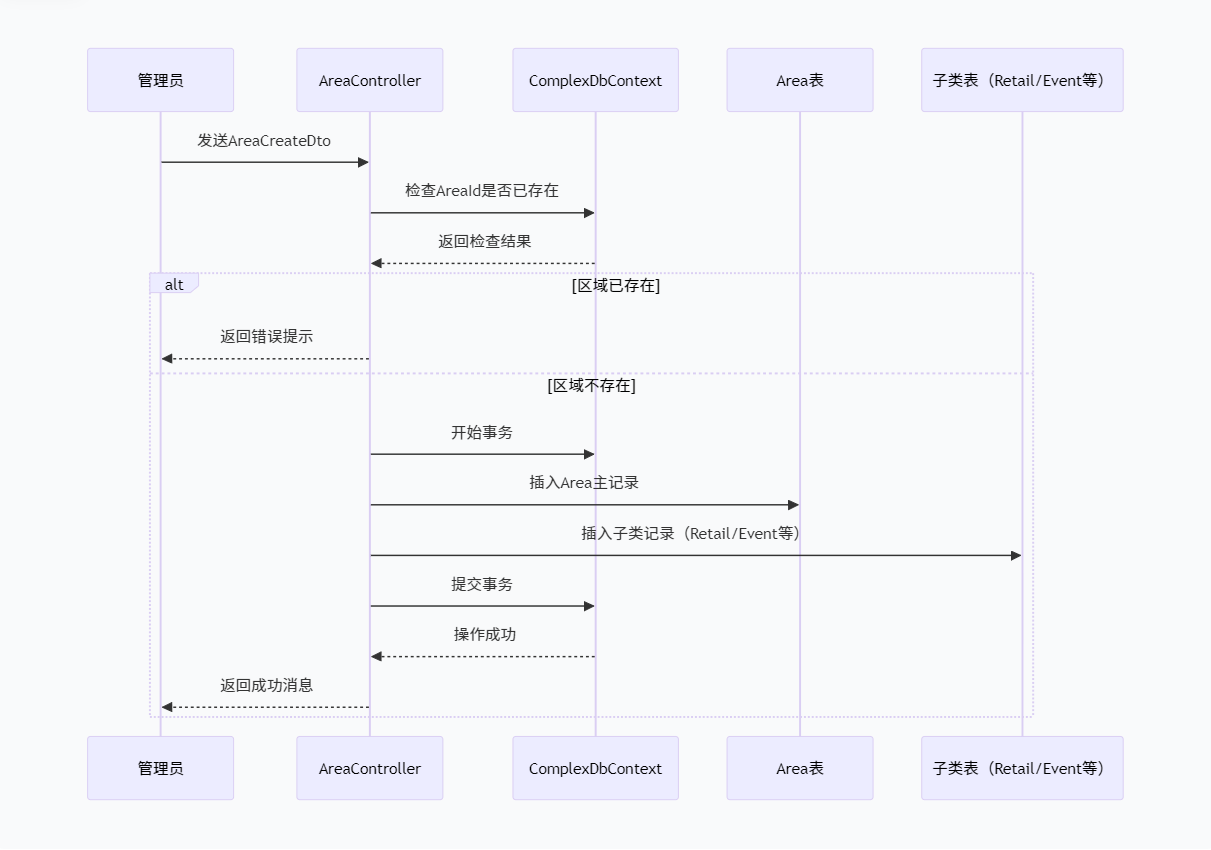
\includegraphics[width=5.64167in,height=2.86458in]{media/media/image_2-3-5.png}

区域信息查询

按类别和空置状态查询:
\begin{verbatim}
[HttpGet("ByCategory")]
public async Task<IActionResult> GetAreas([FromQuery] string? category, [FromQuery] int? isEmpty)
\end{verbatim}
按ID查询:
\begin{verbatim}
[HttpGet("ByID")]
public async Task<IActionResult> GetAreasByID([FromQuery] int id)
\end{verbatim}
用户可根据类别和空置状态查询区域信息。系统返回区域基本信息及其子类特定属性(如租金、容量等)。

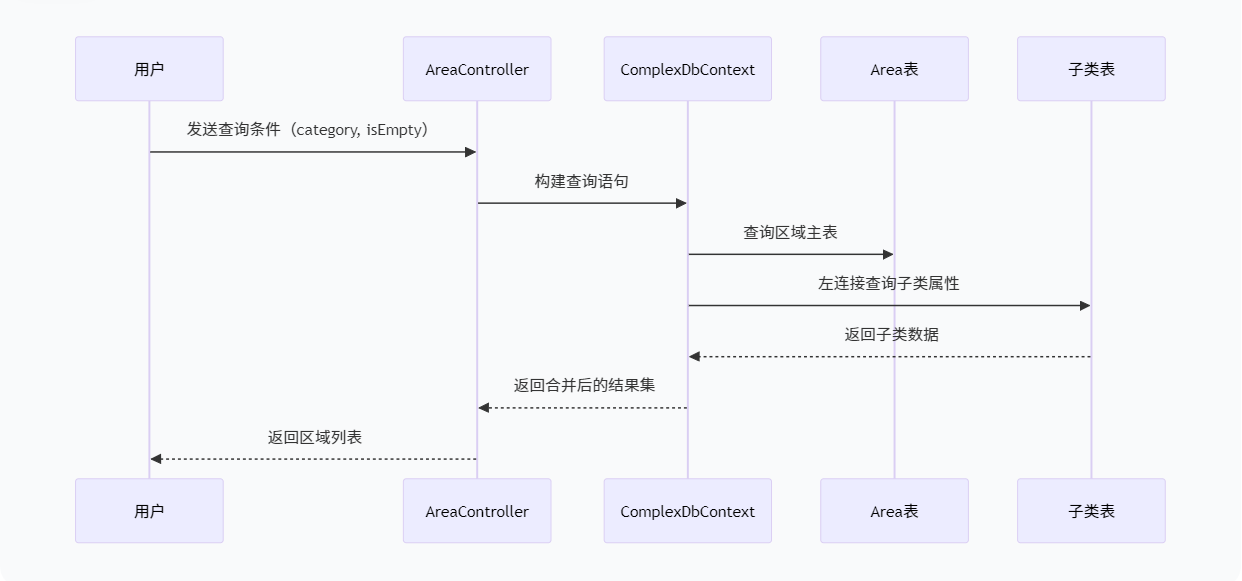
\includegraphics[width=5.64167in,height=2.86458in]{media/media/image_2-3-6.png}

区域信息管理 - 删除

\begin{verbatim}
[HttpDelete("{id}")]
public async Task<IActionResult> DeleteArea(int id)
\end{verbatim}
管理员删除指定区域。系统会检查该区域是否被租用或有关联活动,若无则删除主表和子表记录。

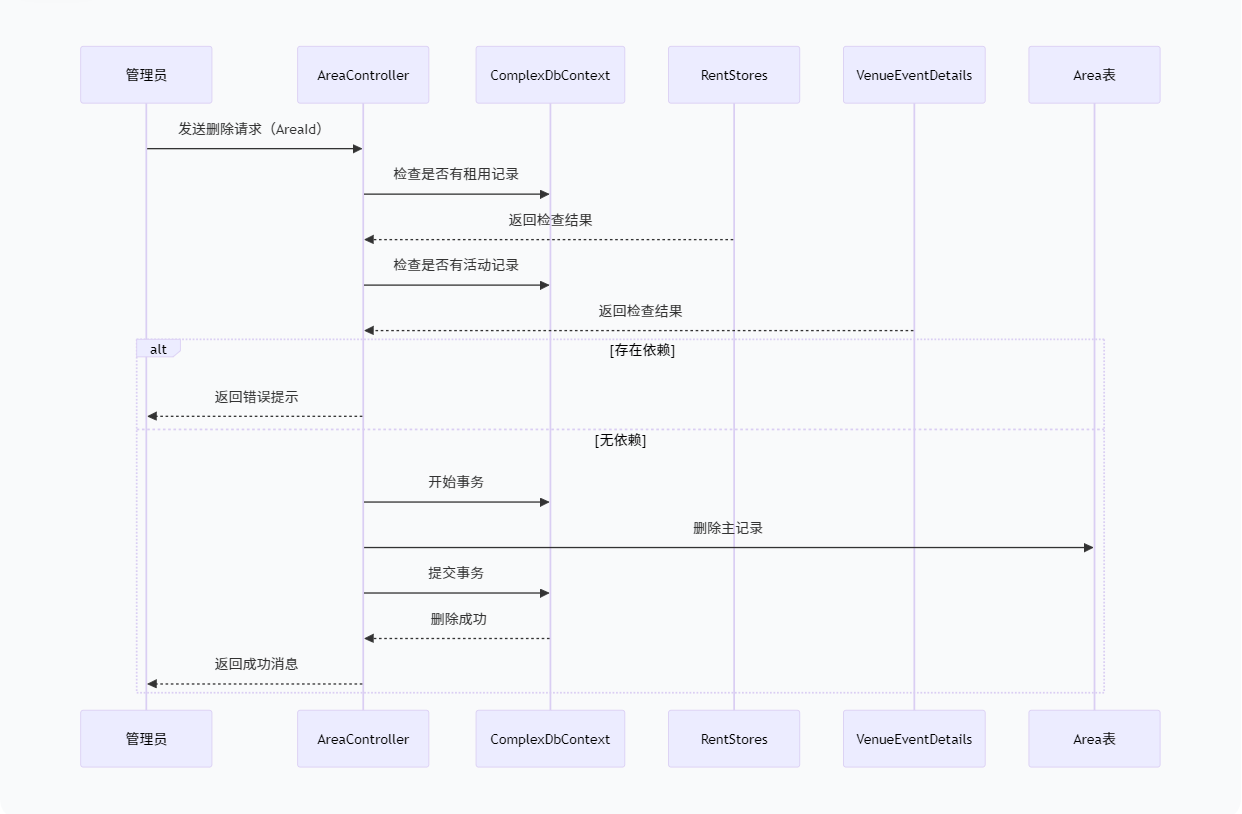
\includegraphics[width=5.64167in,height=2.86458in]{media/media/image_2-3-7.png}

\hypertarget{ux7528ux4f8b-2}{%
  \subsection{合作方用例}\label{ux7528ux4f8b-2}}

\hypertarget{ux7528ux4f8b-2ux8bbeux8ba1}{%
  \subsubsection{合作方用例设计}\label{ux7528ux4f8b-2ux8bbeux8ba1}}

\begin{longtable}[]{@{}ll@{}}
  \toprule
  \textbf{动作序列} & \textbf{描述}                  \\
  \midrule
  \endhead
  添加新合作方        & 在系统内新增一条合作方记录,用于后续场地活动或合作事项  \\
  合作方信息查询       & 项目经理查询合作方的详细信息,用于活动筹备或合作事项跟进 \\
  合作方信息修改       & 项目经理更新合作方的基础信息及关联活动状态        \\
  合作方统计信息报表     & 按时间段生成合作方运营统计报表,支持筛选与导出      \\
  \bottomrule
\end{longtable}

添加新合作方:

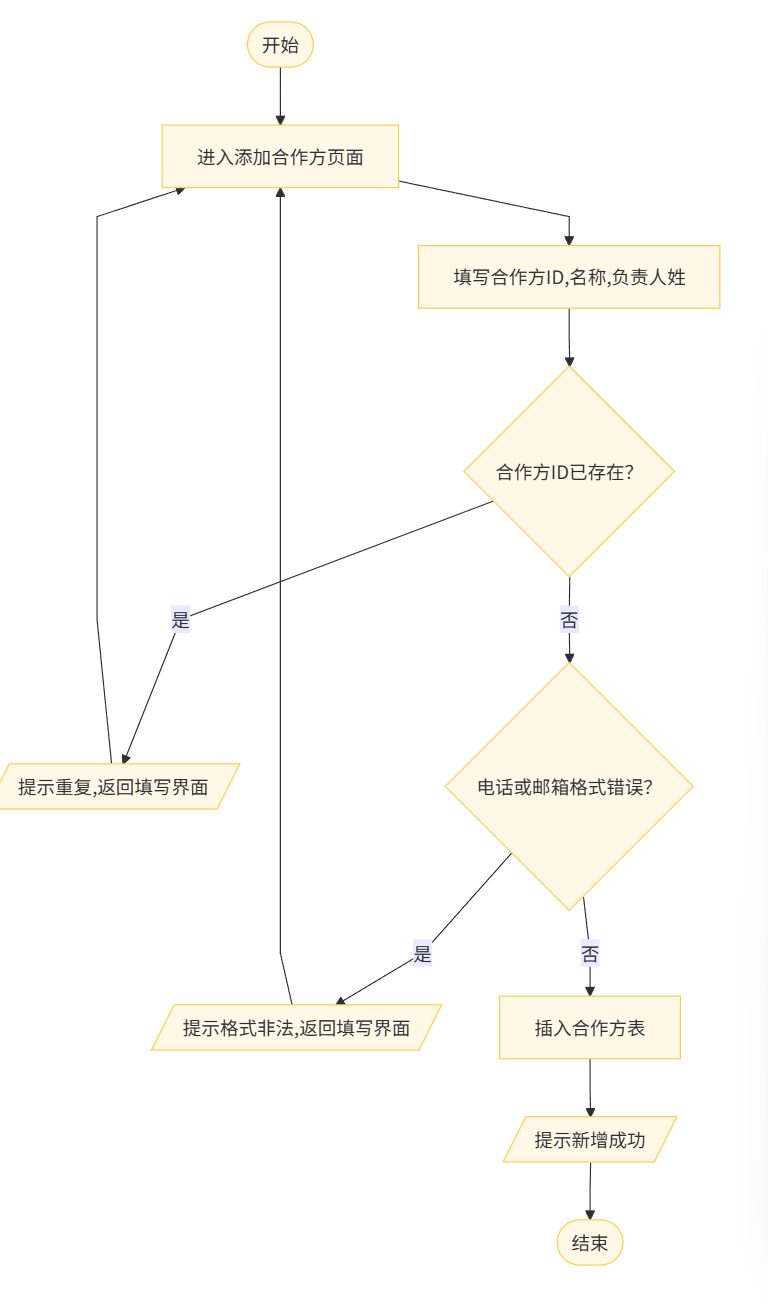
\includegraphics[width=4.45694in,height=4.83819in]{media/media/image_2-4-1.png}

合作方信息查询:

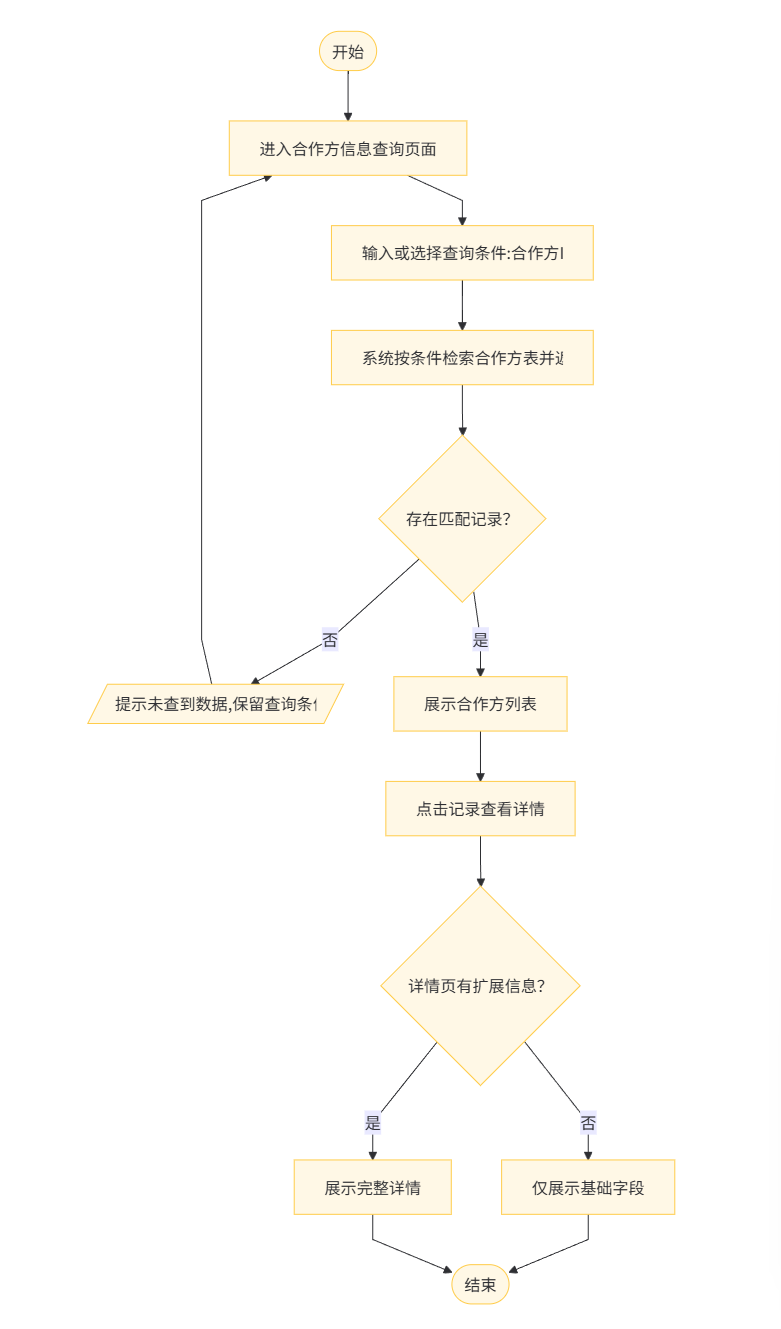
\includegraphics[width=4.45694in,height=4.83819in]{media/media/image_2-4-2.png}

合作方信息修改:

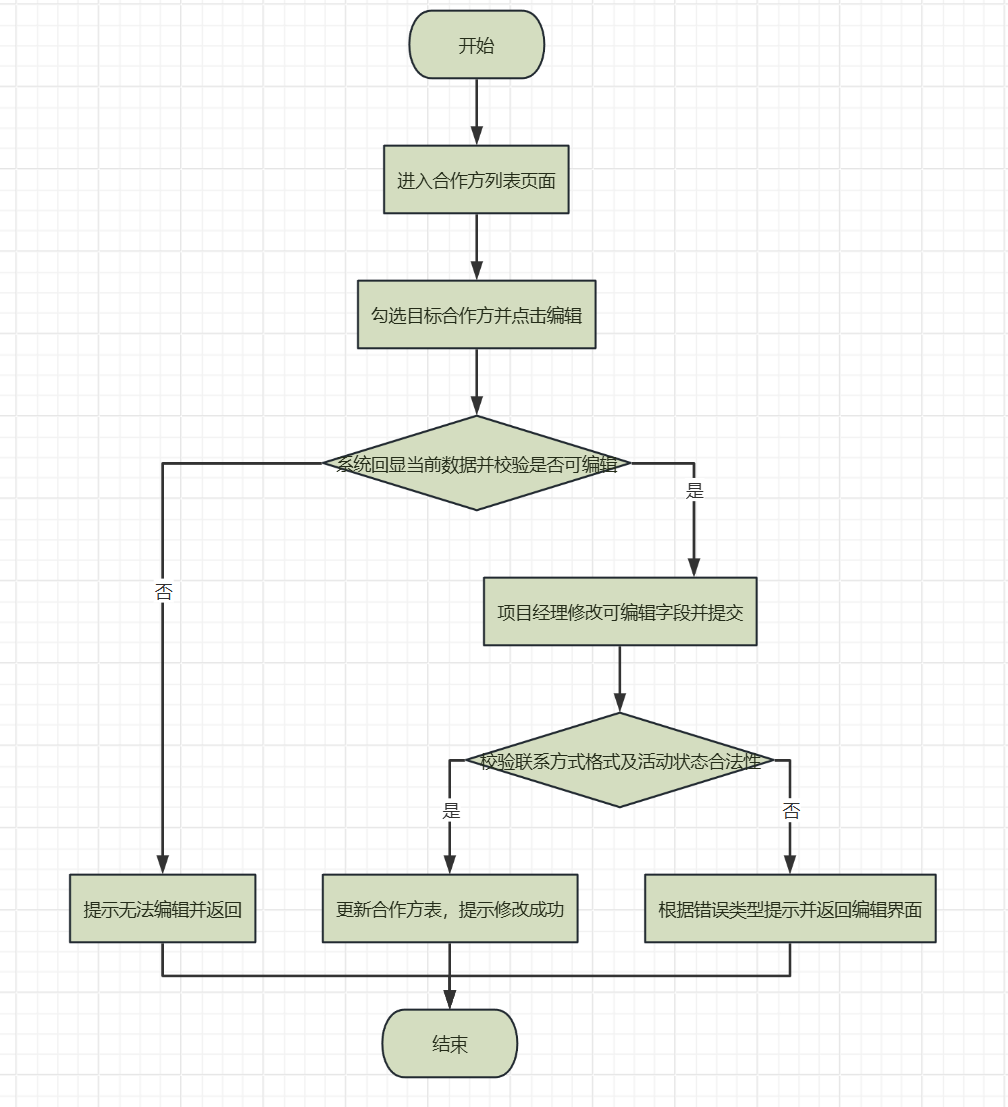
\includegraphics[width=4.45694in,height=4.83819in]{media/media/image_2-4-3.png}

合作方统计信息报表:

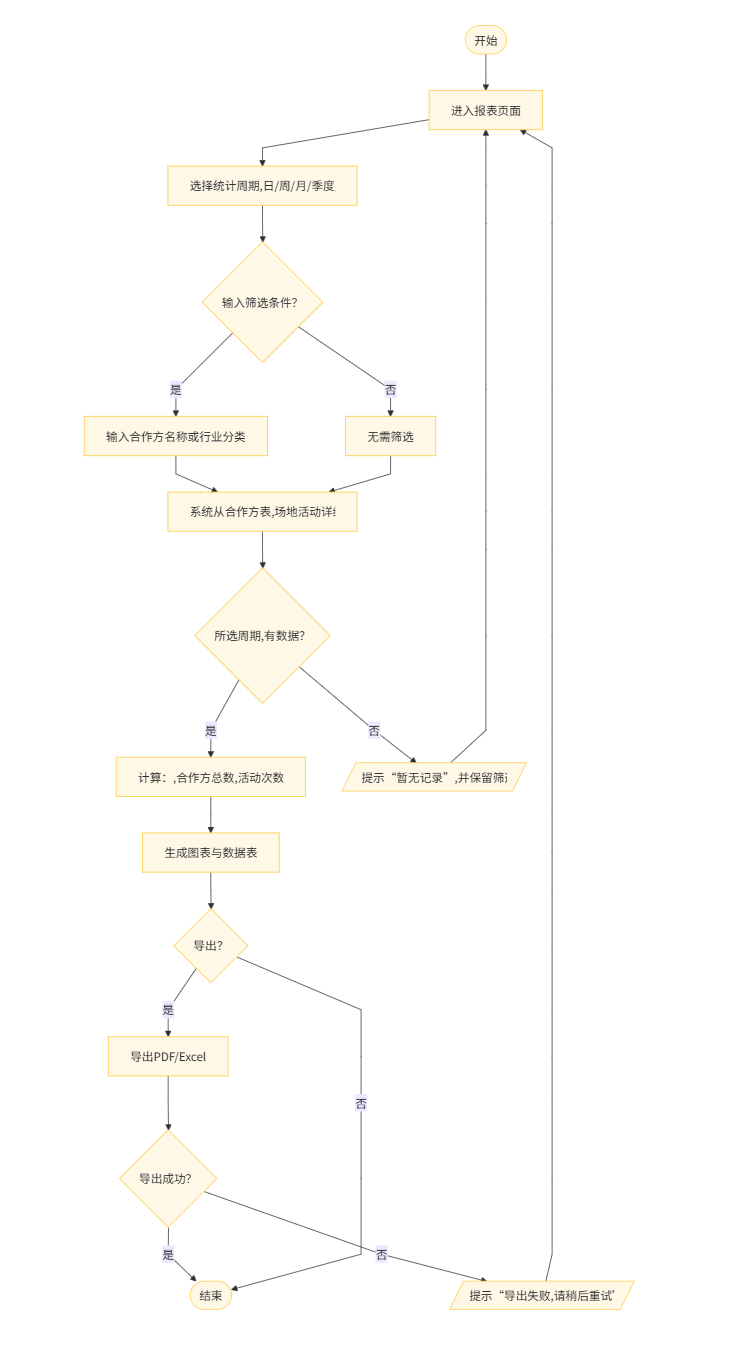
\includegraphics[width=4.45694in,height=4.83819in]{media/media/image_2-4-4.png}


\hypertarget{ux7528ux4f8b-2ux5b9eux73b0}{%
  \subsubsection{合作方用例实现}\label{ux7528ux4f8b-2ux5b9eux73b0}}

合作方用例实现

添加新合作方:

\begin{verbatim}
public class CollaborationDto
{
    [Required(ErrorMessage = "合作方ID是必填项")]
    [Range(1, 99999999999, ErrorMessage = "合作方ID必须大于0,且不能超过11位")]
    public int CollaborationId { get; set; }

    [Required(ErrorMessage = "合作方名称是必填项")]
    [StringLength(50, ErrorMessage = "名称长度不能超过50个字符")]
    public string CollaborationName { get; set; }

    [StringLength(50, ErrorMessage = "联系人姓名长度不能超过50个字符")]
    public string Contactor { get; set; }

    [Phone(ErrorMessage = "无效的电话号码格式")]
    [StringLength(20, ErrorMessage = "电话号码长度不能超过20个字符")]
    public string PhoneNumber { get; set; }

    [EmailAddress(ErrorMessage = "无效的电子邮件格式")]
    [StringLength(50, ErrorMessage = "电子邮件长度不能超过50个字符")]
    public string Email { get; set; }
}
[HttpPost]
public async Task<IActionResult> AddCollaboration(
    [FromQuery, Required] string operatorAccountId,
    [FromBody] CollaborationDto dto)
\end{verbatim}

首先验证操作员是否具有数据库管理员权限(1),然后检查提供的合作方ID是否已存在。如果ID唯一,则创建新的合作方实体并保存到数据库,同时记录操作日志。用于系统管理员添加新的合作方信息,确保合作方数据的唯一性和完整性,为后续的场馆活动合作提供基础数据支持。

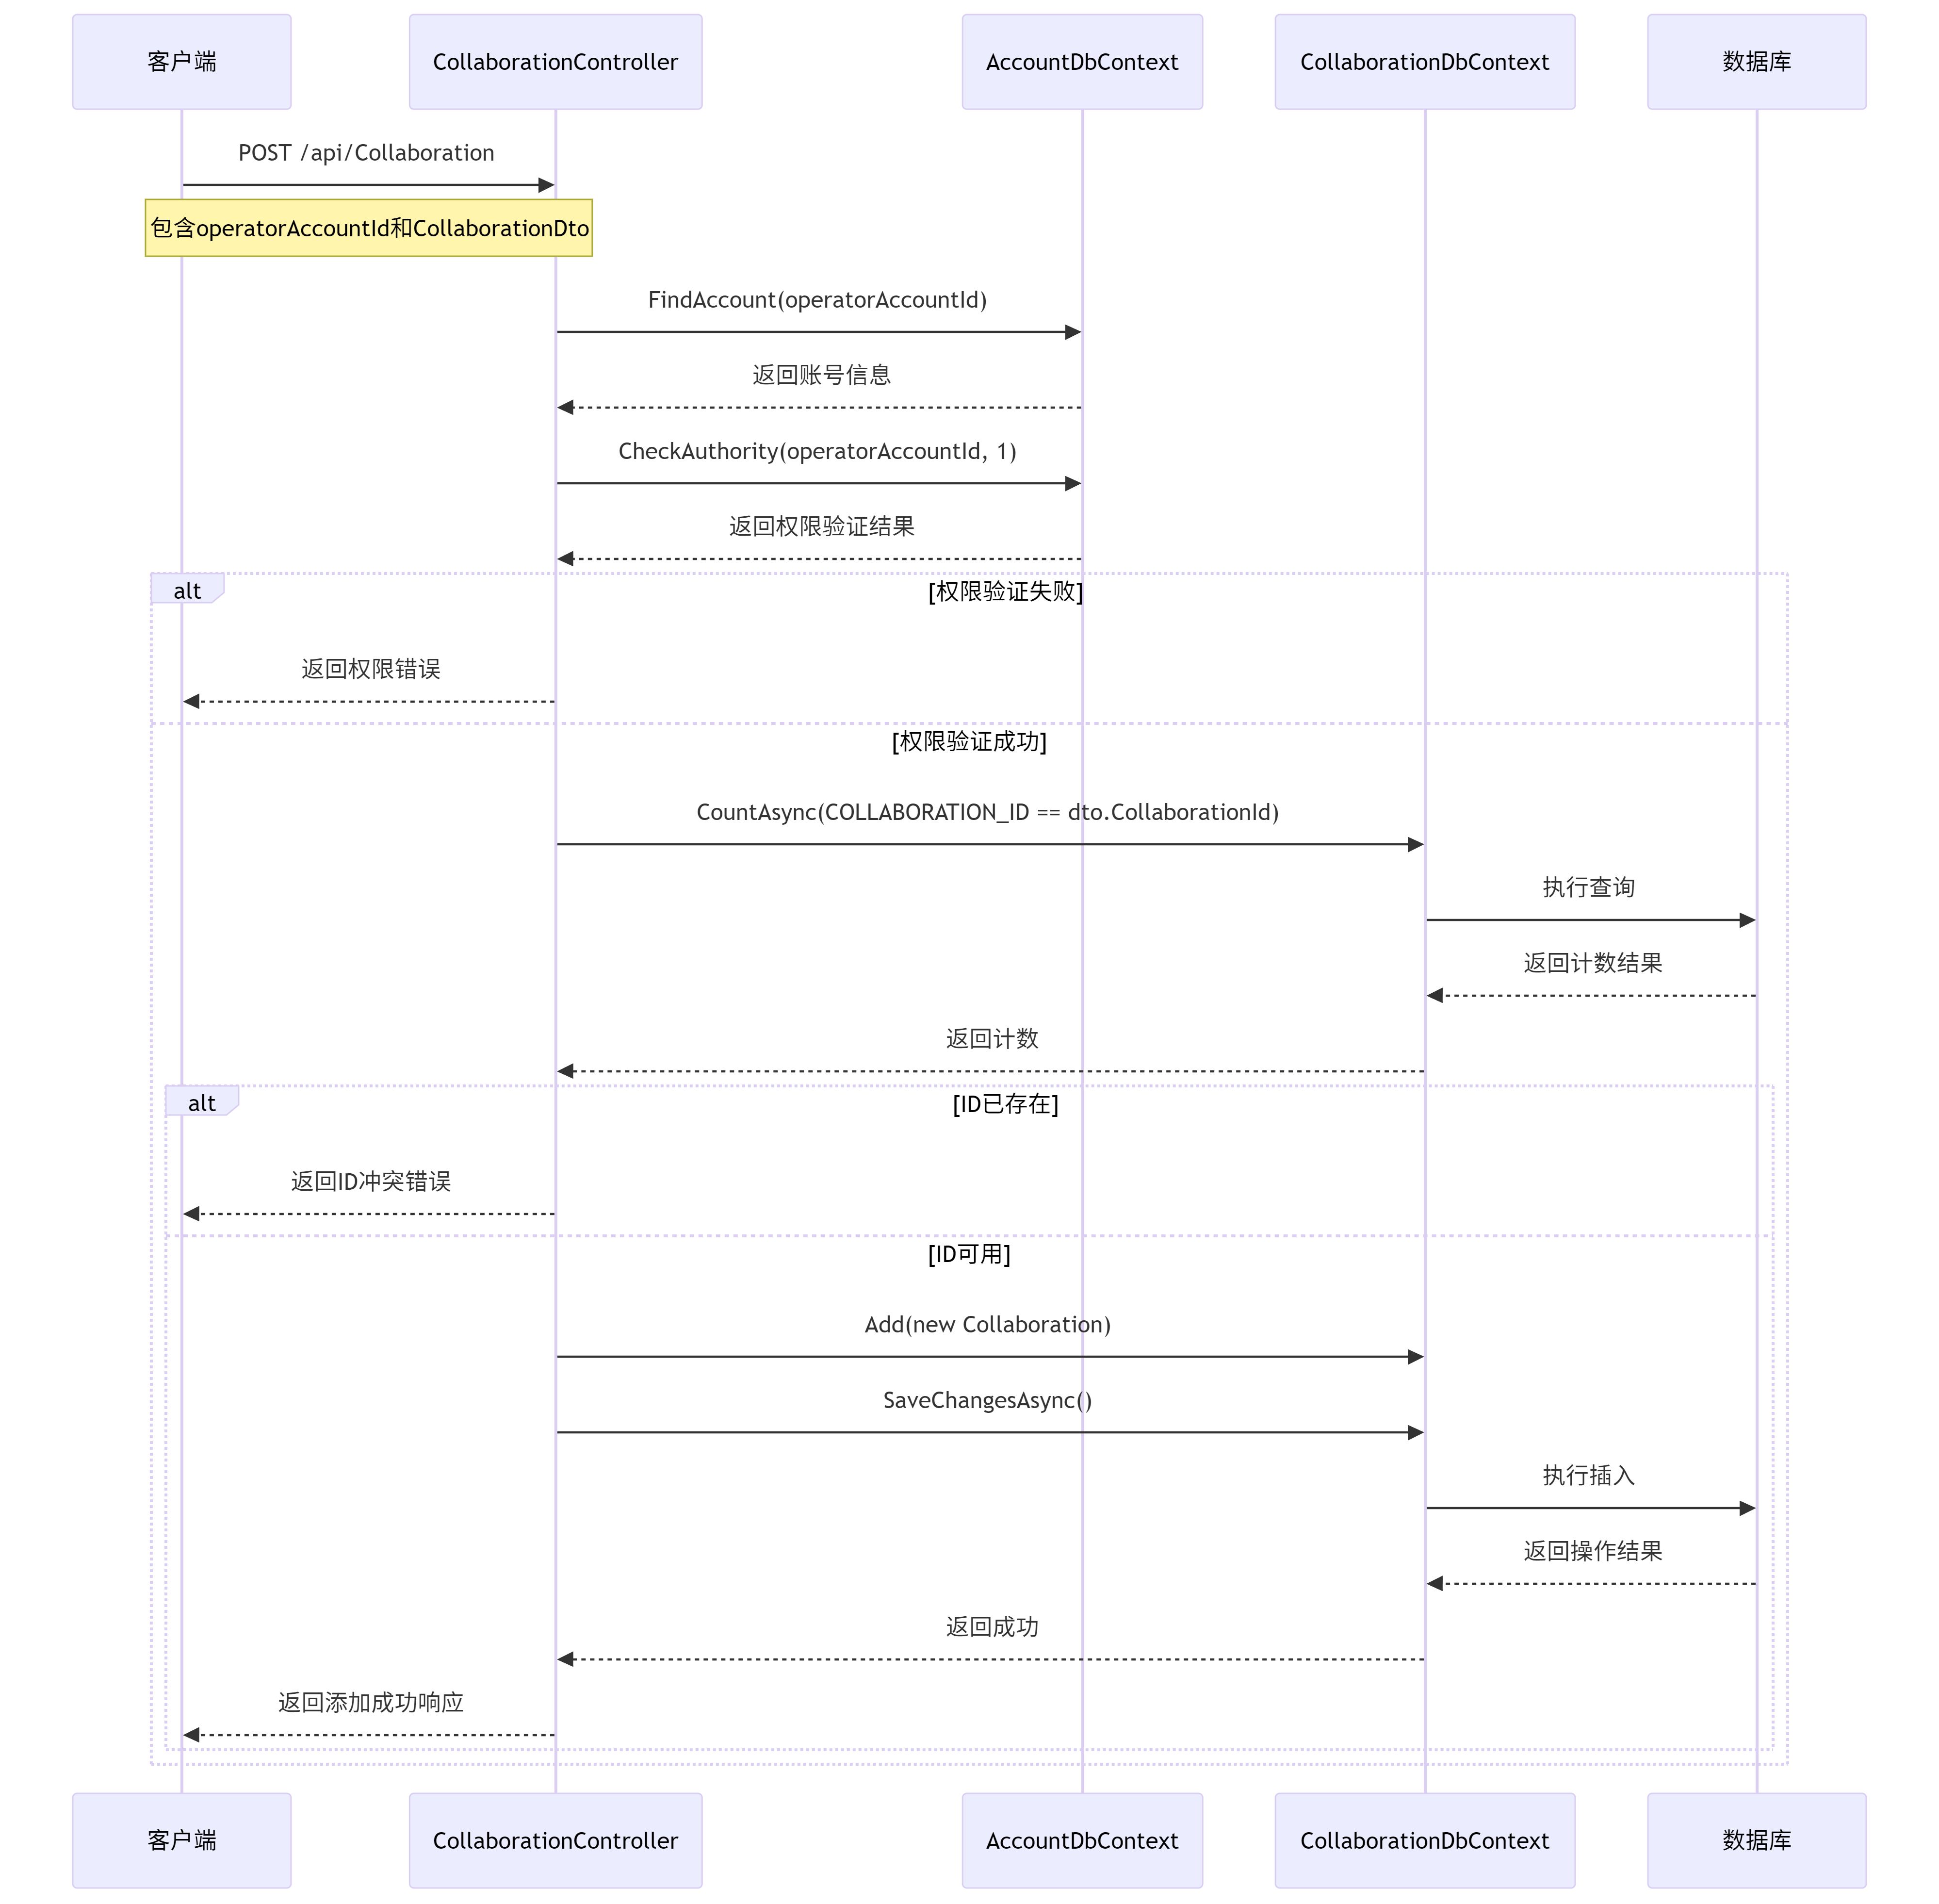
\includegraphics[width=5.64167in,height=2.86458in]{media/media/image_2-4-5.png}

合作方信息查询:

\begin{verbatim}
[HttpGet]
public async Task<IActionResult> SearchCollaborations(
    [FromQuery, Required] string operatorAccountId,
    [FromQuery] int? id,
    [FromQuery] string? name,
    [FromQuery] string? contactor)
\end{verbatim}

验证操作员是否具有数据库管理员(1)或部门经理权限(2),然后根据提供的查询条件(ID、名称或联系人)构建动态查询,返回匹配的合作方列表。为管理人员提供灵活的合作方信息检索功能,支持按多种条件筛选,便于快速查找特定合作方信息。

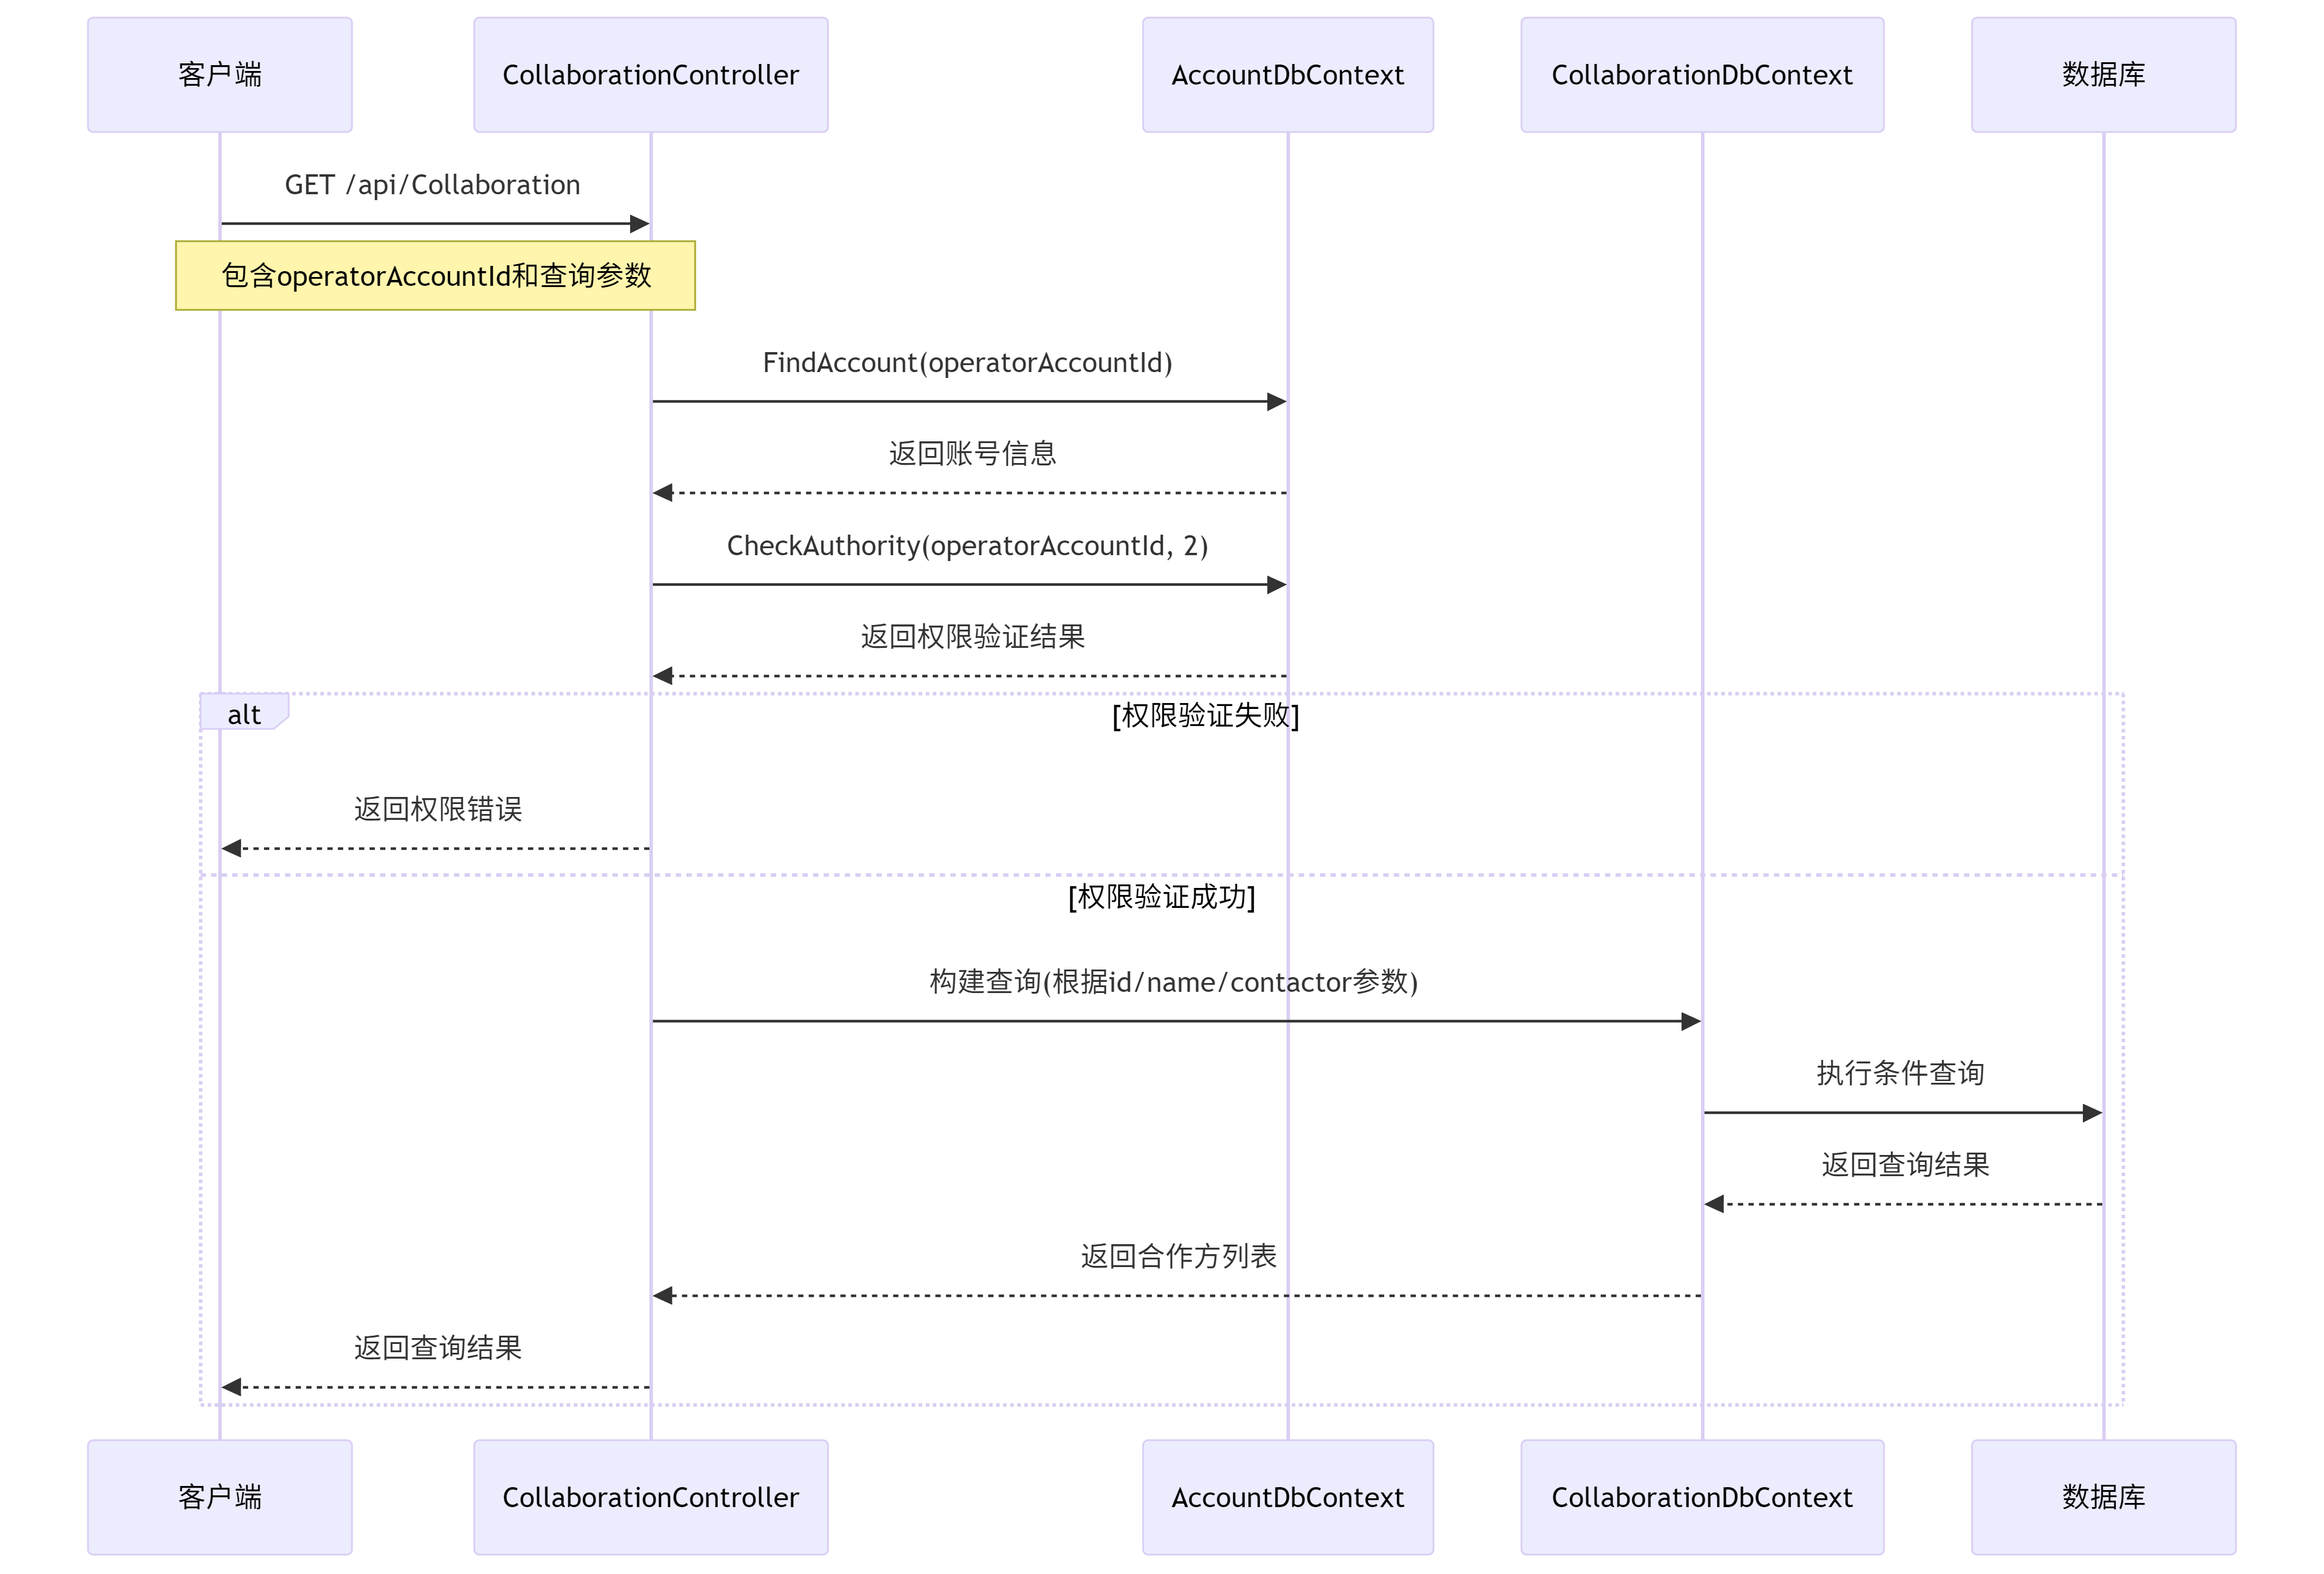
\includegraphics[width=5.64167in,height=2.86458in]{media/media/image_2-4-6.png}

合作方信息修改:

\begin{verbatim}
public class CollaborationUpdateDto
{
    [StringLength(50, ErrorMessage = "名称长度不能超过50个字符")]
    public string CollaborationName { get; set; }

    [StringLength(50, ErrorMessage = "联系人姓名长度不能超过50个字符")]
    public string Contactor { get; set; }

    [Phone(ErrorMessage = "无效的电话号码格式")]
    [StringLength(20, ErrorMessage = "电话号码长度不能超过20个字符")]
    public string PhoneNumber { get; set; }

    [EmailAddress(ErrorMessage = "无效的电子邮件格式")]
    [StringLength(50, ErrorMessage = "电子邮件长度不能超过50个字符")]
    public string Email { get; set; }
}
[HttpPut("{id}")]
public async Task<IActionResult> UpdateCollaboration(
    int id, 
    [FromQuery, Required] string operatorAccountId,
    [FromBody] CollaborationUpdateDto dto)
\end{verbatim}

验证操作员是否具有数据库管理员权限(1),检查目标合作方是否存在以及是否正在进行活动(存在活动则不允许修改)。若可修改,则更新合作方的可修改字段并保存更改。允许系统管理员维护合作方信息的准确性,确保合作方数据的时效性,同时防止对正在进行活动的合作方造成干扰。

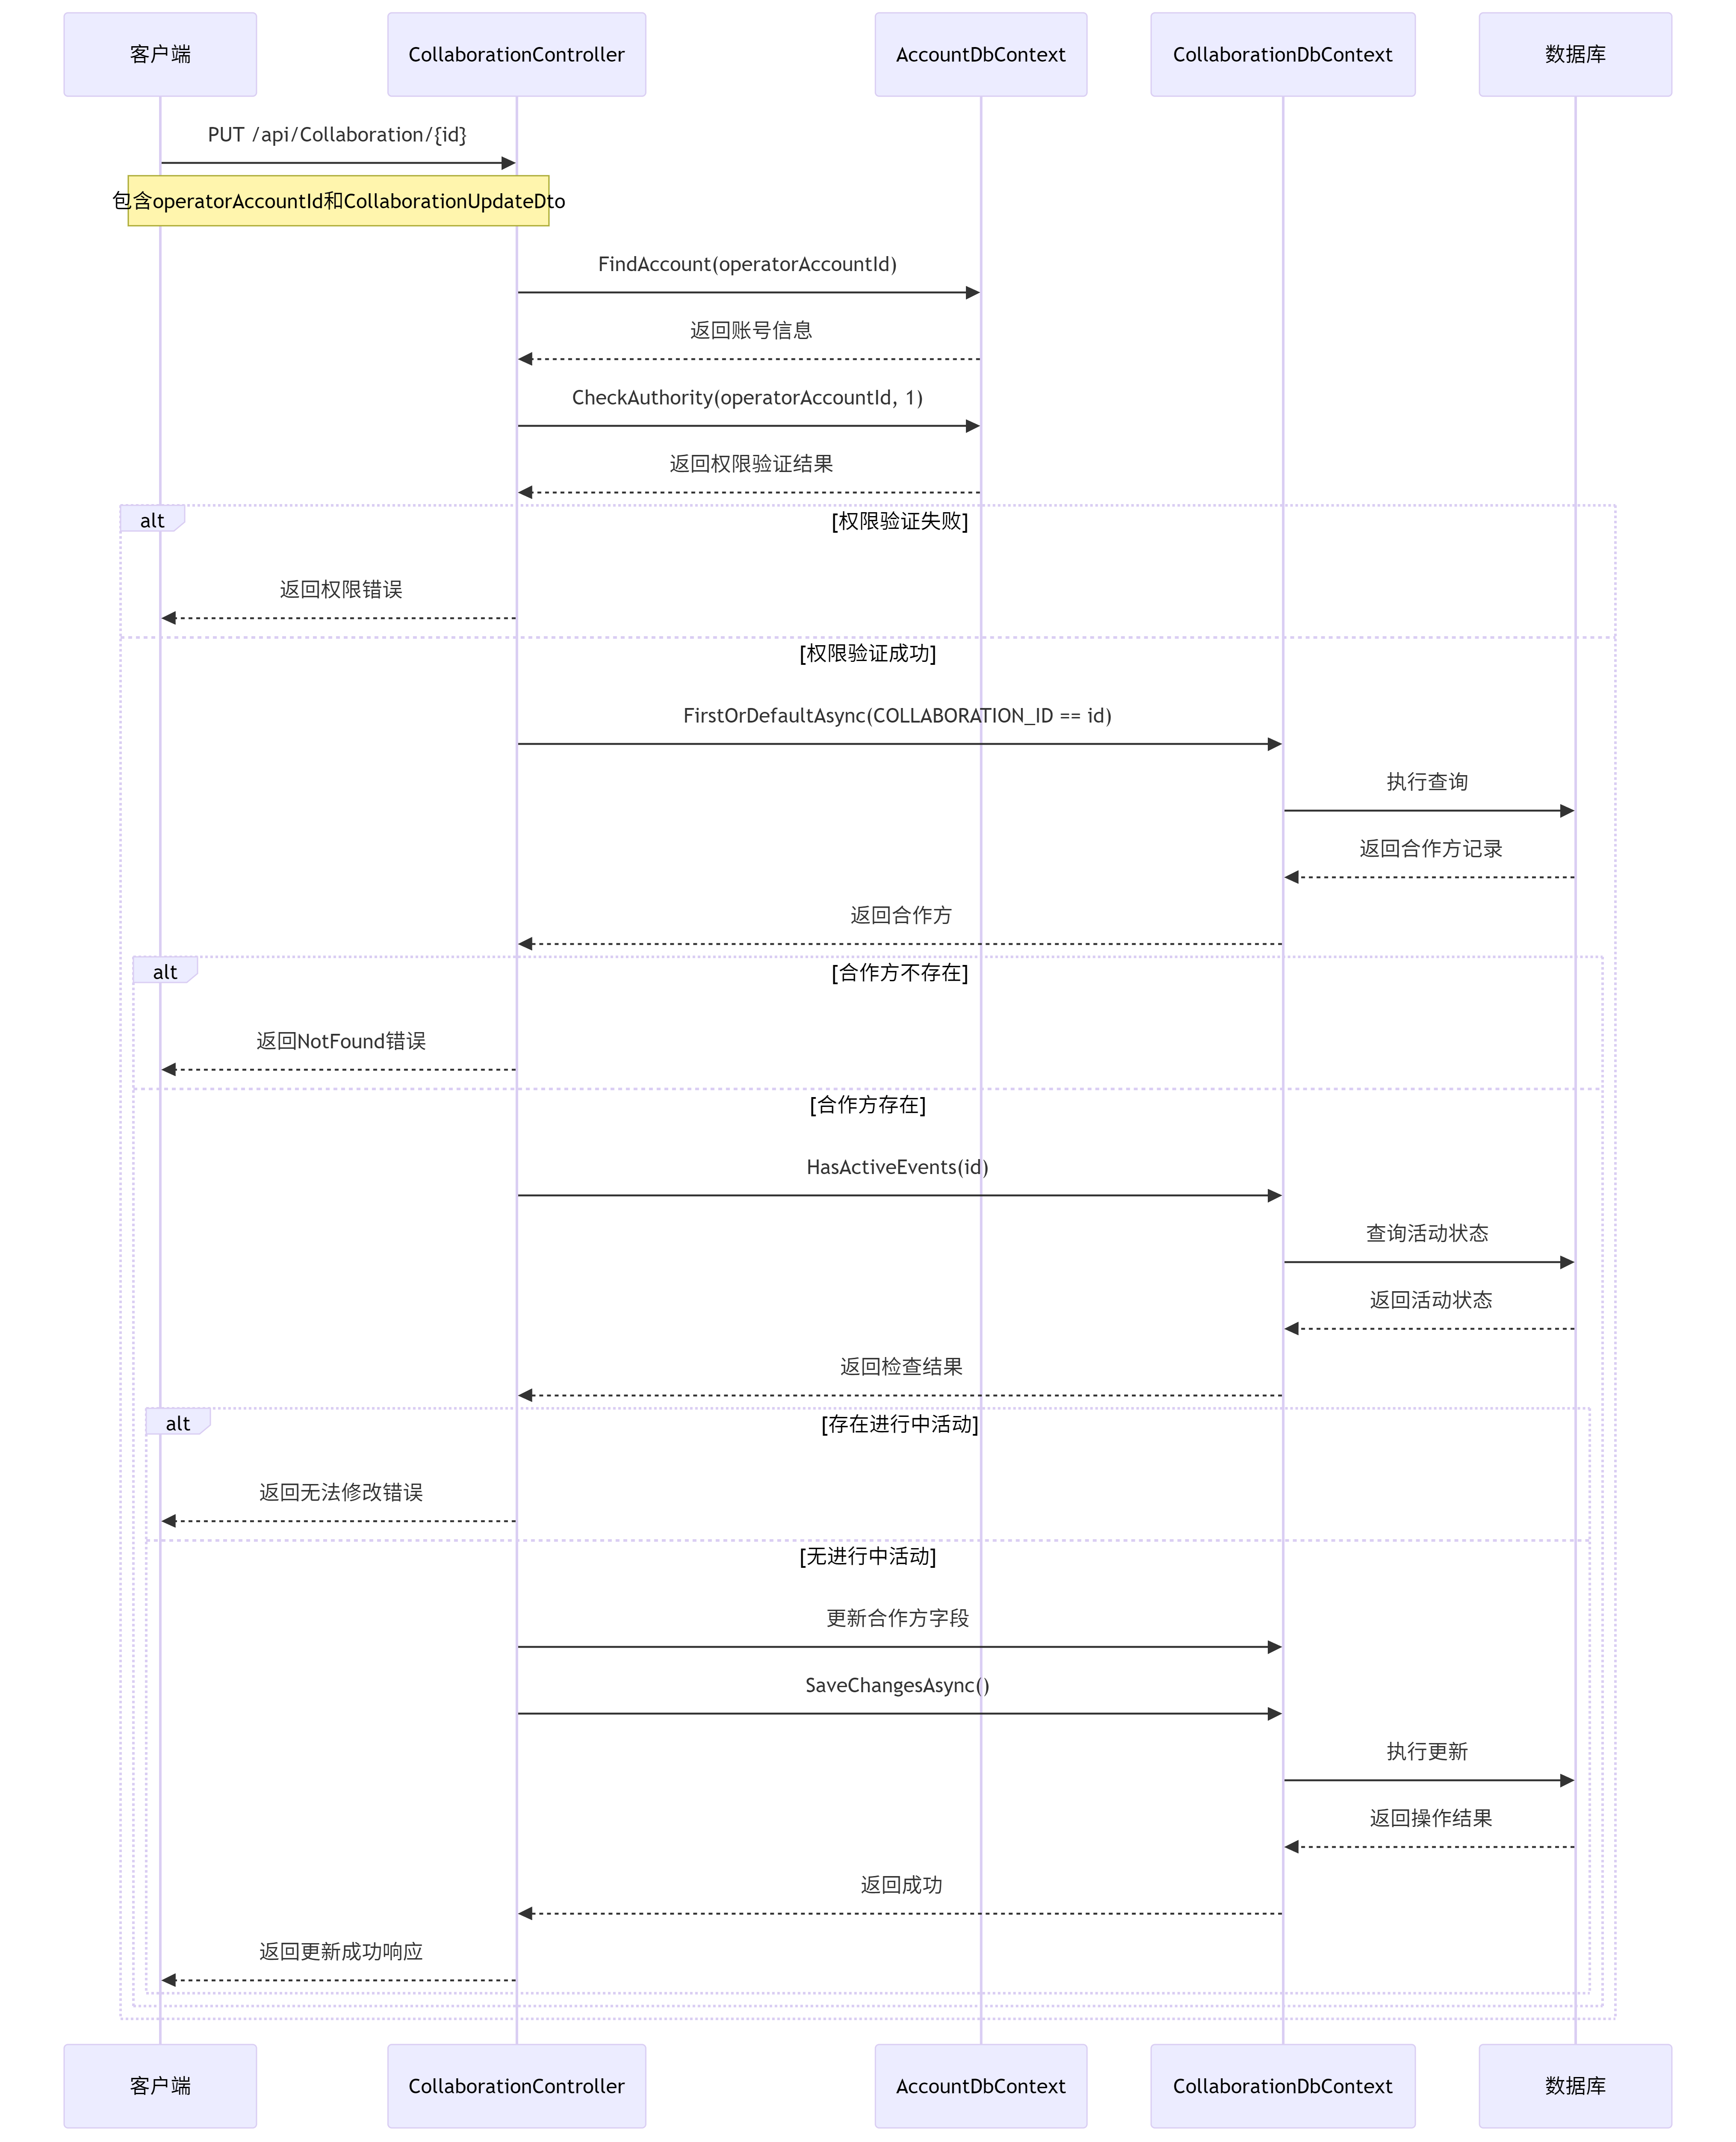
\includegraphics[width=5.64167in,height=2.86458in]{media/media/image_2-4-7.png}

合作方统计信息报表:

\begin{verbatim}
[HttpGet("report")]
public async Task<IActionResult> GenerateReport(
    [FromQuery, Required] string operatorAccountId,
    [FromQuery] DateTime startDate,
    [FromQuery] DateTime endDate,
    [FromQuery] string? industry)
\end{verbatim}

验证操作员权限(需要权限1或2),验证时间范围的合理性,然后按时间范围和行业筛选条件统计各合作方的活动数量、总投资和平均收益。为管理层提供合作方业务活动的统计分析数据,支持决策制定,帮助评估不同合作方的贡献度和投资回报率

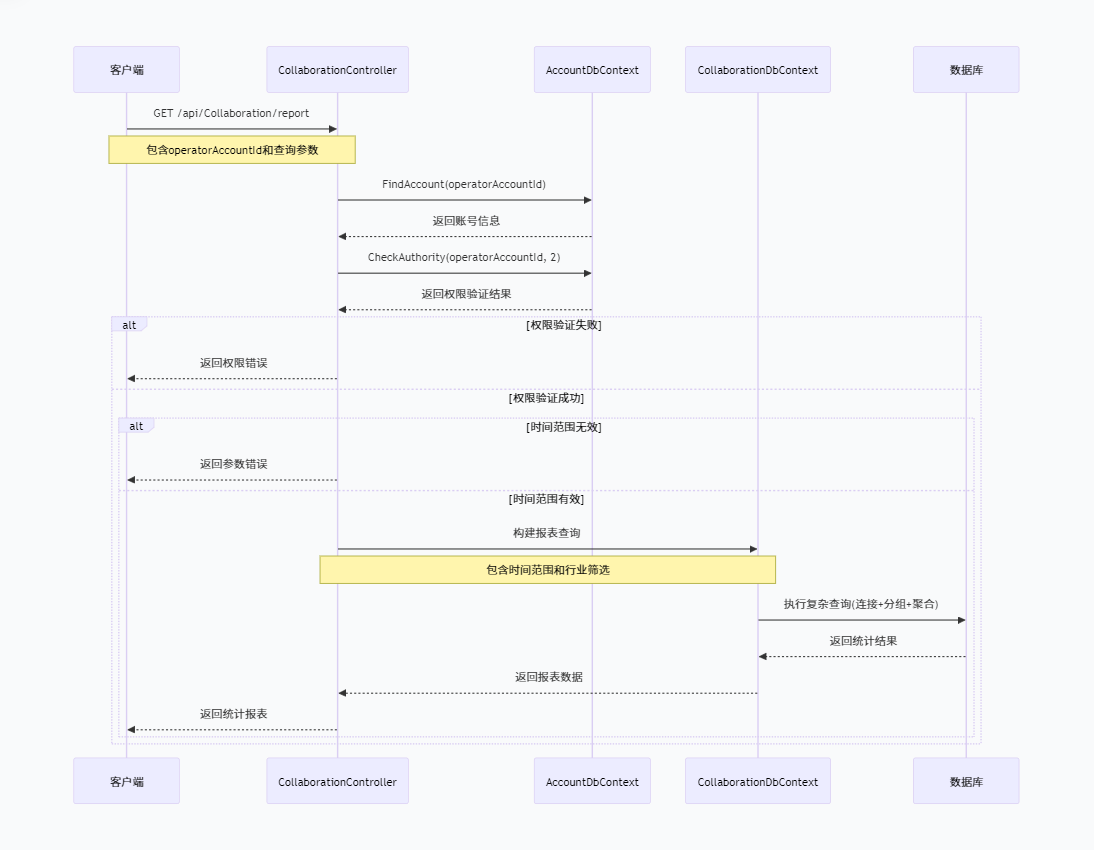
\includegraphics[width=5.64167in,height=2.86458in]{media/media/image_2-4-8.png}

\hypertarget{ux7528ux4f8b-3}{%
  \subsection{**用例}\label{ux7528ux4f8b-3}}

\hypertarget{ux5458ux5de5ux7528ux4f8b}{%
  \subsection{员工用例}\label{ux5458ux5de5ux7528ux4f8b}}

\hypertarget{ux5458ux5de5ux7528ux4f8bux8bbeux8ba1}{%
  \subsubsection{员工用例设计}\label{ux5458ux5de5ux7528ux4f8bux8bbeux8ba1}}

表格 2‑6 员工功能的动作序列

\begin{longtable}[]{@{}ll@{}}
  \toprule
  动作序列         & 描述\tabularnewline
  \midrule
  \endhead
  添加新员工        & 管理员创建员工账号并分配基础权限。\tabularnewline
  员工权限管理       & 管理人员调整员工的长期权限\tabularnewline
  员工个人信息修改     &
  员工修改个人可编辑信息,管理人员可修改下属的更多信息\tabularnewline
  员工工资管理       & 对员工工资进行管理\tabularnewline
  员工工资统计报表生成功能 &
  系统按部门、时间等维度生成员工工资统计报表\tabularnewline
  员工临时权限管理     & 为员工授予 /
  收回与特定活动相关的临时权限\tabularnewline
  \bottomrule
\end{longtable}

添加员工活动图:

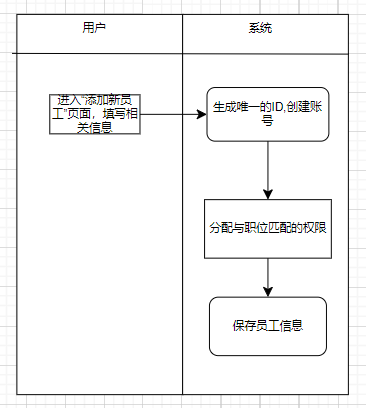
\includegraphics[width=3.10417in,height=3.45694in]{media/media/image8.png}

员工权限管理活动图:

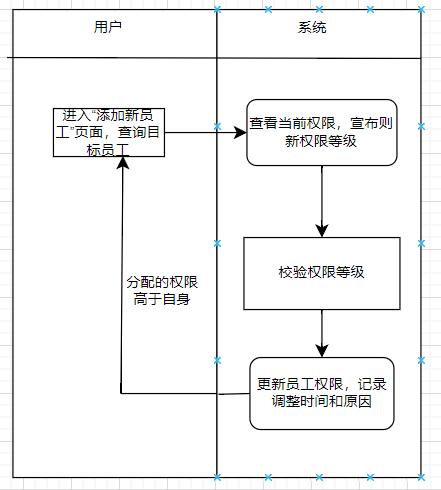
\includegraphics[width=2.95972in,height=3.28333in]{media/media/image9.png}

员工个人信息修改活动图:

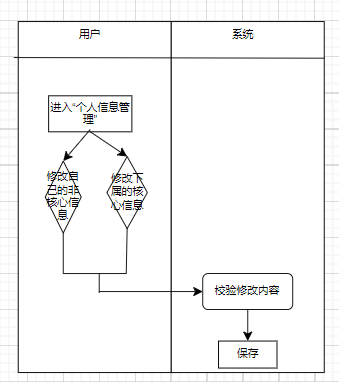
\includegraphics[width=3.53194in,height=3.98264in]{media/media/image10.png}

员工工资管理活动图:

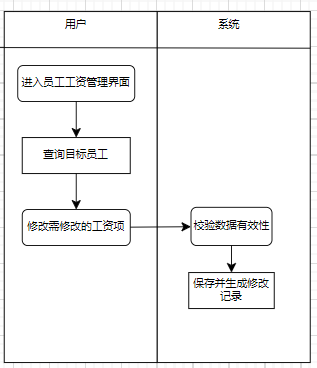
\includegraphics[width=3.02917in,height=3.51458in]{media/media/image11.png}

员工工资统计报表生成活动图:

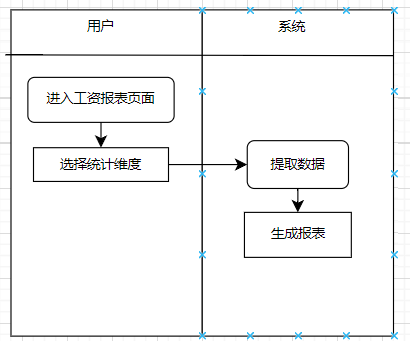
\includegraphics[width=2.90764in,height=2.41597in]{media/media/image12.png}

员工临时权限管理活动图:

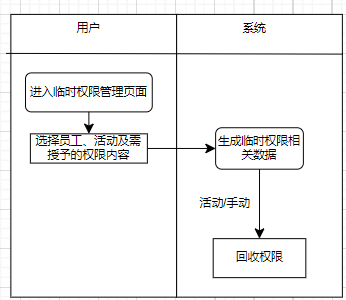
\includegraphics[width=3.075in,height=2.66458in]{media/media/image13.png}

\hypertarget{ux5458ux5de5ux7528ux4f8bux5b9eux73b0}{%
  \subsubsection{员工用例实现}\label{ux5458ux5de5ux7528ux4f8bux5b9eux73b0}}

1. 主要类及其关系:

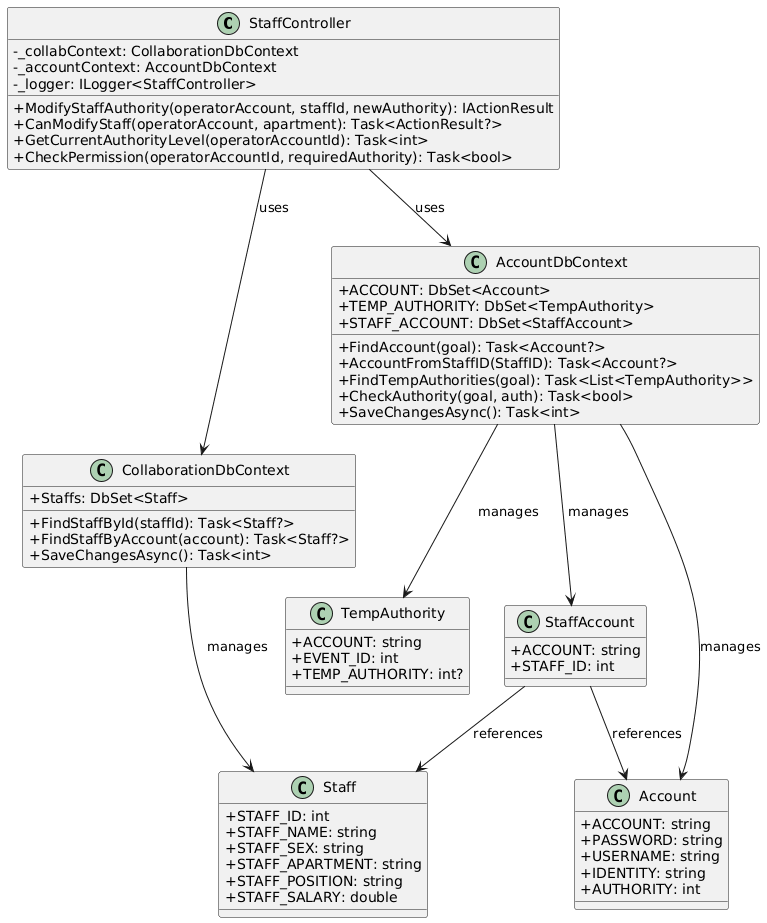
\includegraphics[width=6.23958in,height=7.50903in]{media/media/image14.png}

2. 方法设计与实现:

添加员工:

~ ~ ~ ~ public class StaffDto

~ ~ ~ ~ \{

~ ~ ~ ~ ~ ~ {[}Required(ErrorMessage = "员工姓名是必填项"){]}

~ ~ ~ ~ ~ ~ {[}StringLength(50, ErrorMessage =
"名称长度不能超过50个字符"){]}

~ ~ ~ ~ ~ ~ public string STAFF\_NAME \{ get; set; \}

~ ~ ~ ~ ~ ~ {[}StringLength(10, ErrorMessage =
"性别长度不能超过10个字符"){]}

~ ~ ~ ~ ~ ~ public string STAFF\_SEX \{ get; set; \}

~ ~ ~ ~ ~ ~ {[}Required(ErrorMessage = "员工部门是必填项"){]}

~ ~ ~ ~ ~ ~ {[}StringLength(50, ErrorMessage =
"部门长度不能超过50个字符"){]}

~ ~ ~ ~ ~ ~ public string STAFF\_APARTMENT \{ get; set; \}

~ ~ ~ ~ ~ ~ {[}Required(ErrorMessage = "员工职位是必填项"){]}

~ ~ ~ ~ ~ ~ {[}StringLength(50, ErrorMessage =
"职位长度不能超过50个字符"){]}

~ ~ ~ ~ ~ ~ public string STAFF\_POSITION \{ get; set; \}

~ ~ ~ ~ ~ ~ {[}Required(ErrorMessage = "员工薪资是必填项"){]}

~ ~ ~ ~ ~ ~ {[}Range(0, 9999999999.99, ErrorMessage =
"薪资必须大于等于0,且不能超过10位整数和2位小数"){]}

~ ~ ~ ~ ~ ~ public double STAFF\_SALARY \{ get; set; \}

~ ~ ~ ~ \}

~ ~ ~ ~ {[}HttpPost("AddStaff"){]}

~ ~ ~ ~ public async Task\textless{}IActionResult\textgreater{}
AddStaff(

~ ~ ~ ~ ~ ~ {[}FromQuery, Required{]} string operatorAccount,

~ ~ ~ ~ ~ ~ {[}FromBody{]} StaffDto dto)

~ ~ ~ ~ \{

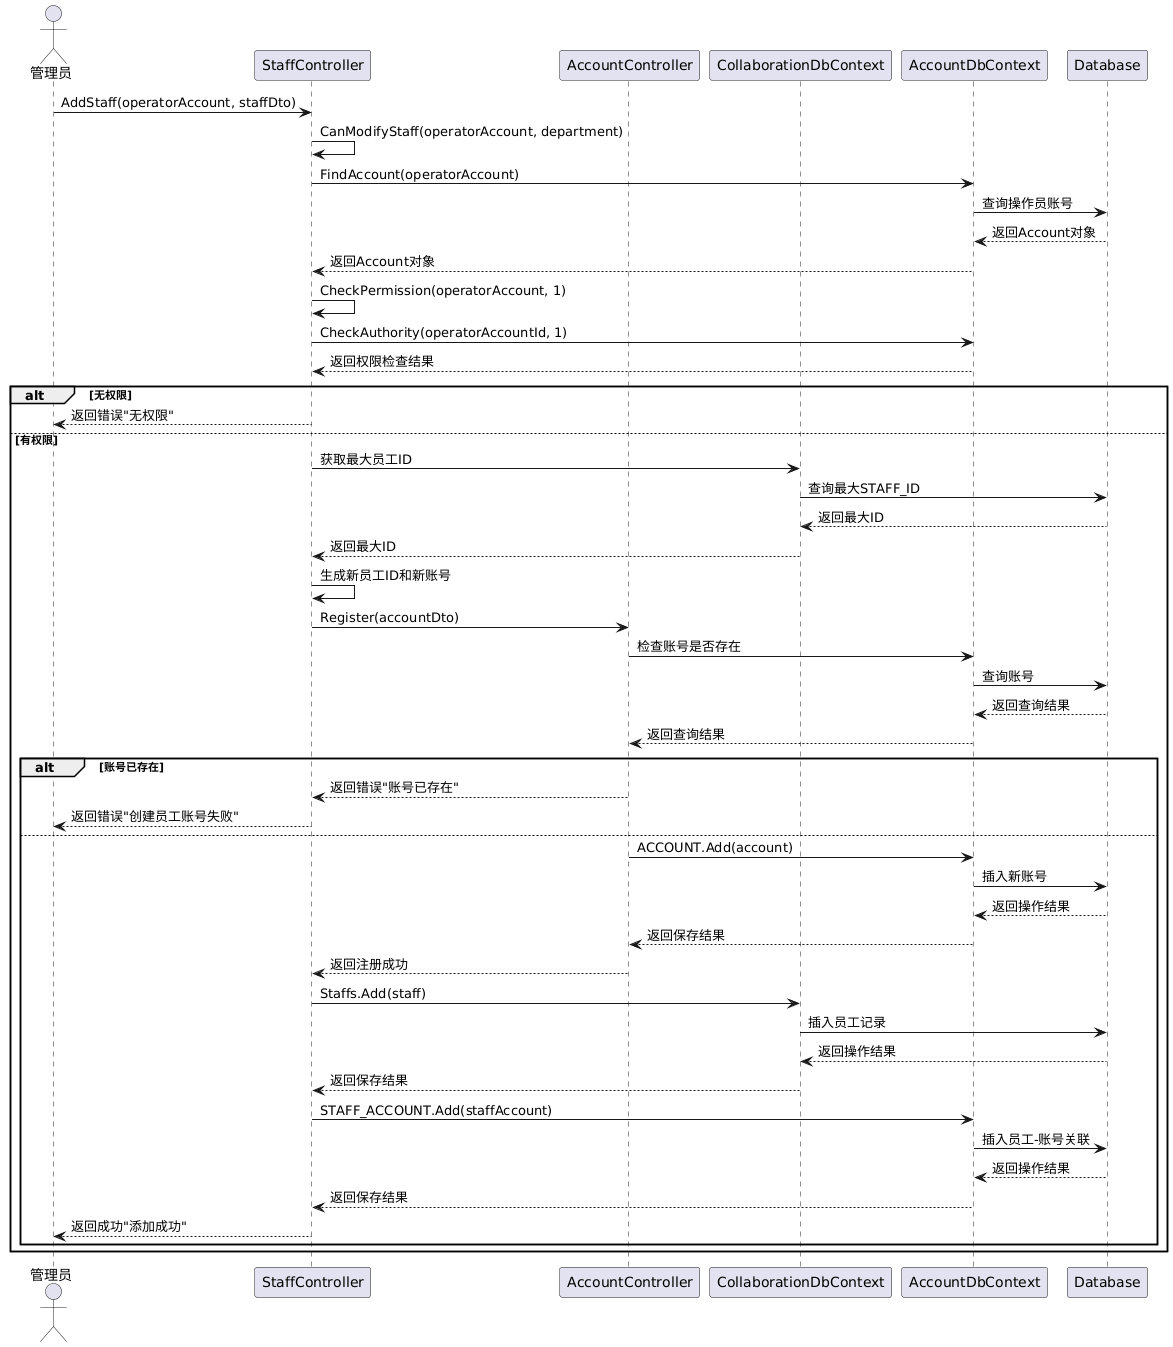
\includegraphics[width=6.27778in,height=7.20903in]{media/media/image15.png}

员工权限管理:

~ ~ ~ ~ {[}HttpPatch("ModifyStaffAuthority"){]}

~ ~ ~ ~ public async Task\textless{}IActionResult\textgreater{}
ModifyStaffAuthority(

~ ~ ~ ~ ~ ~ {[}FromQuery, Required{]} string operatorAccount,

~ ~ ~ ~ ~ ~ {[}FromQuery{]} int staffId,

~ ~ ~ ~ ~ ~ {[}FromQuery{]} int newAuthority)

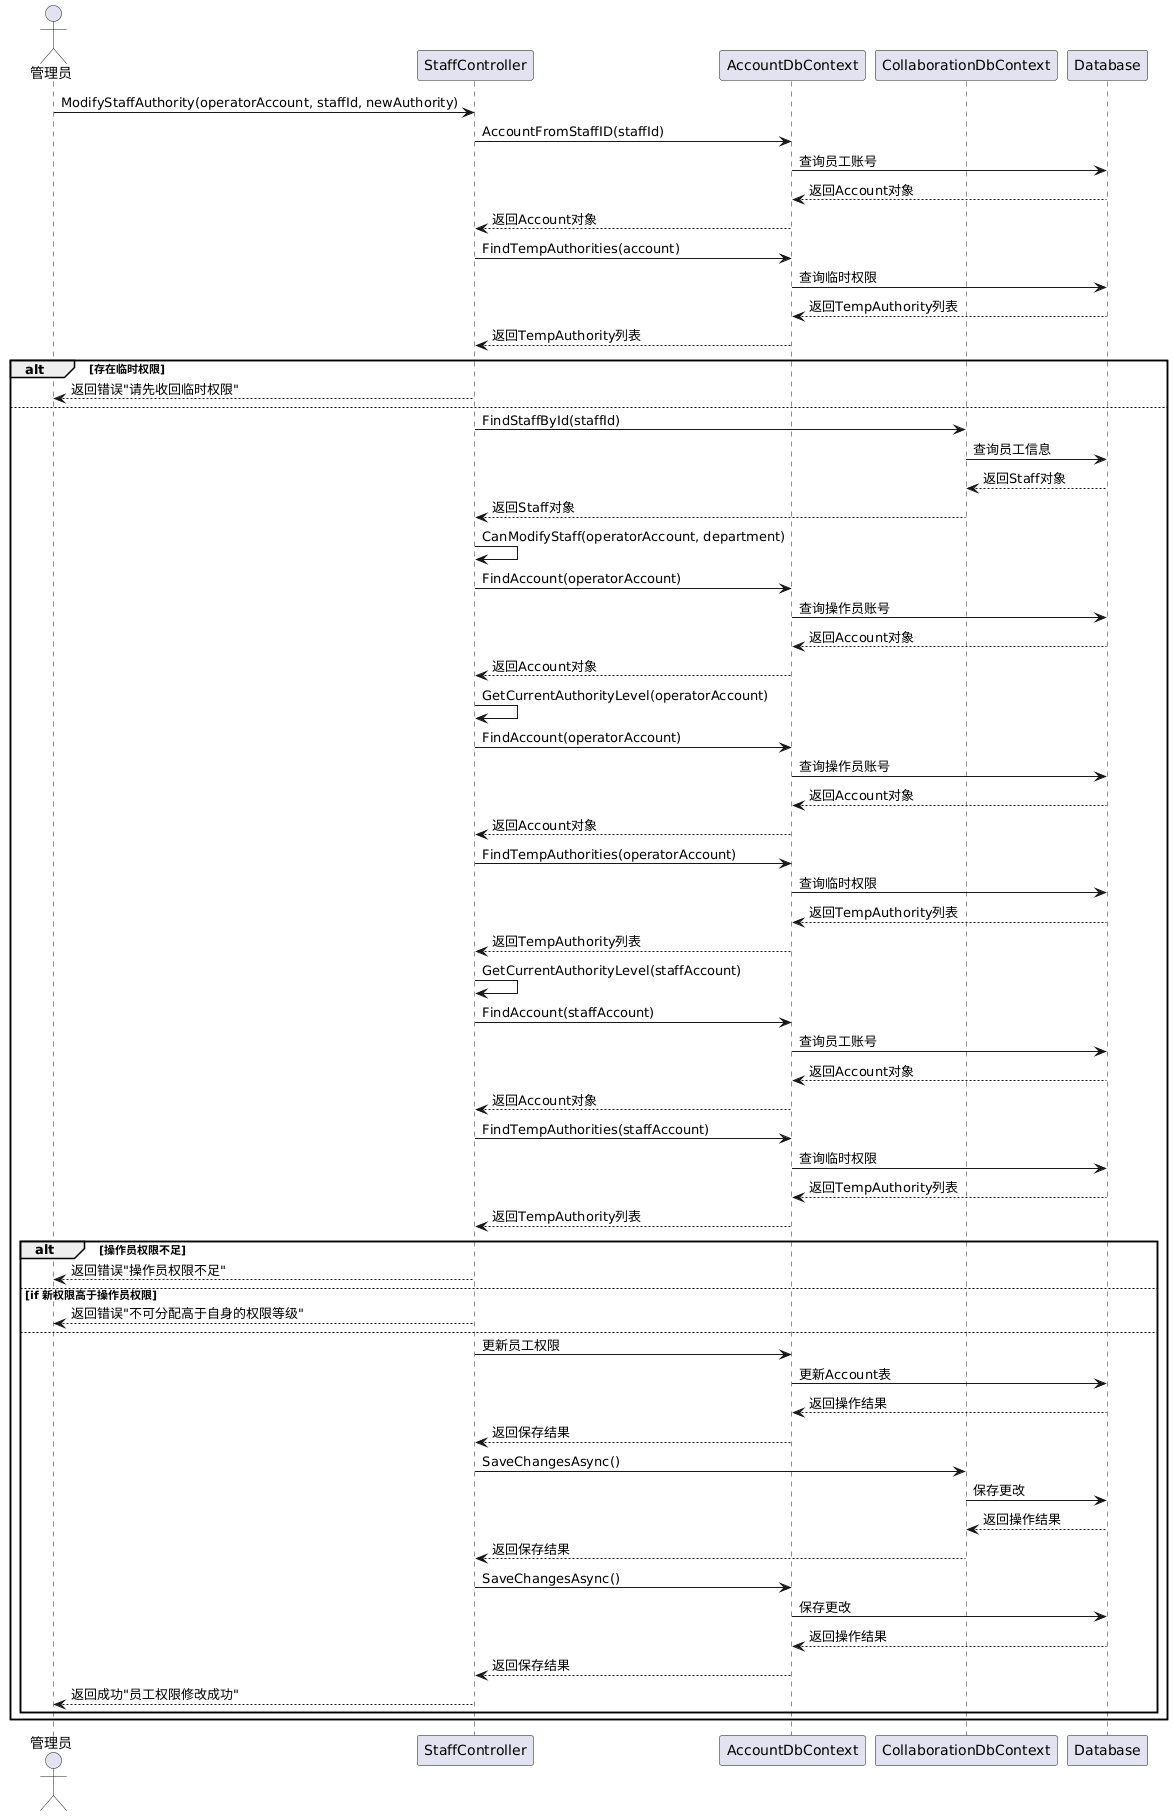
\includegraphics[width=5.98403in,height=9.26389in]{media/media/image16.png}

员工修改信息:

~ ~ ~ ~ {[}HttpPatch("ModifyStaffInfo"){]}

~ ~ ~ ~ public async Task\textless{}IActionResult\textgreater{}
UpdateStaff(

~ ~ ~ ~ ~ ~ {[}FromQuery, Required{]} int staffId,

~ ~ ~ ~ ~ ~ {[}FromQuery, Required{]} string operatorAccount,

~ ~ ~ ~ ~ ~ {[}FromBody{]} StaffDto dto)

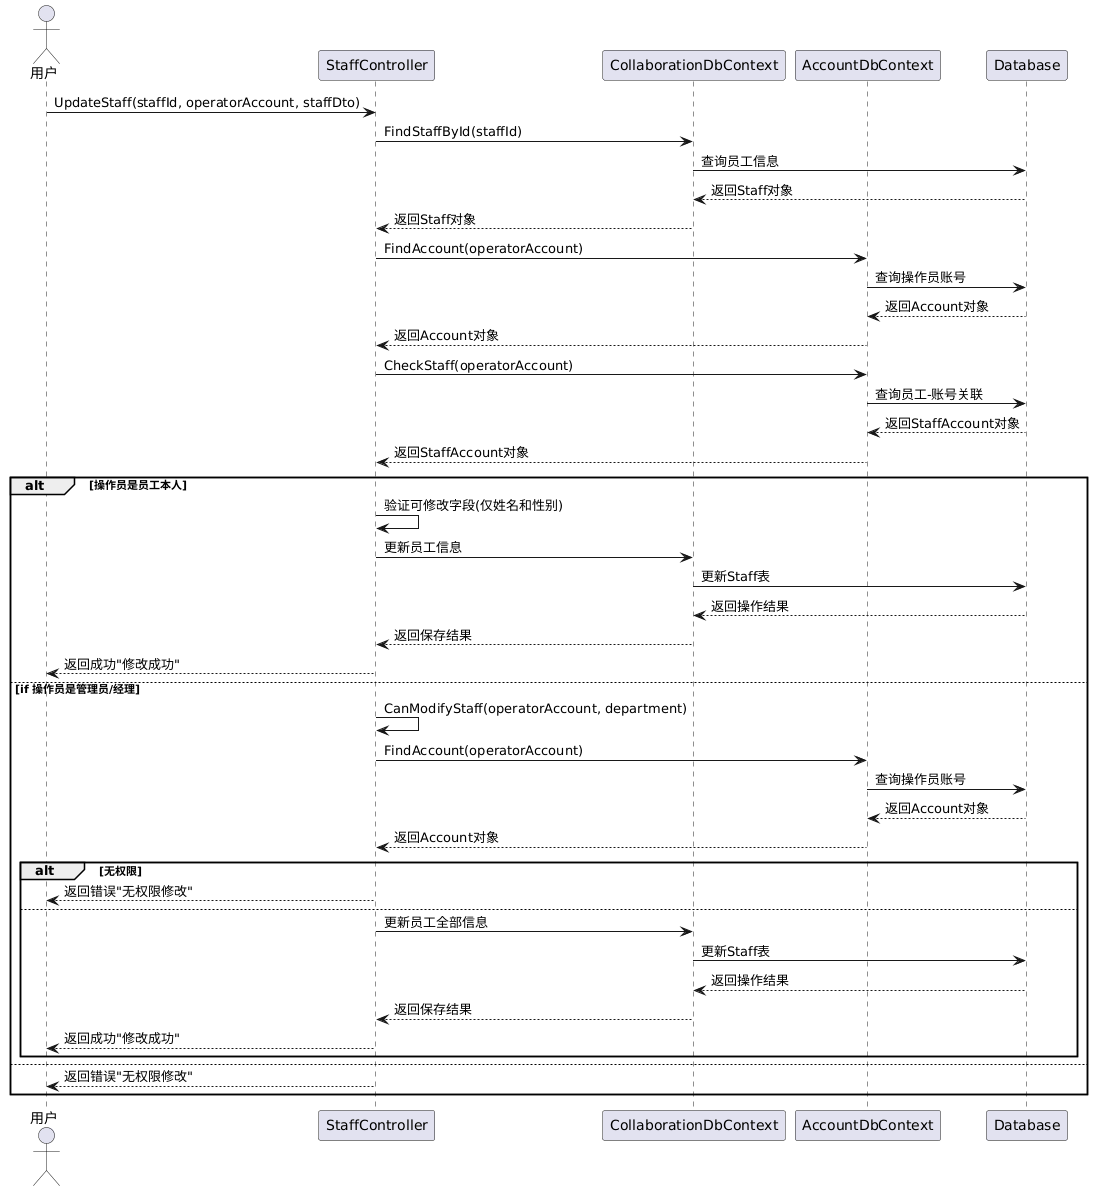
\includegraphics[width=6.20625in,height=6.7625in]{media/media/image17.png}

员工工资管理:

~ ~ ~ ~ {[}HttpPost("StaffSalaryManagement"){]}

~ ~ ~ ~ public async Task\textless{}IActionResult\textgreater{}
ManageStaffSalary(

~ ~ ~ ~ ~ ~ {[}FromQuery, Required{]} string operatorAccount,

~ ~ ~ ~ ~ ~ {[}FromQuery, Required{]} int staffId,

~ ~ ~ ~ ~ ~ {[}FromQuery{]} DateTime monthTime, // 格式 如 2008-11

~ ~ ~ ~ ~ ~ {[}FromBody{]} SalaryDto dto)

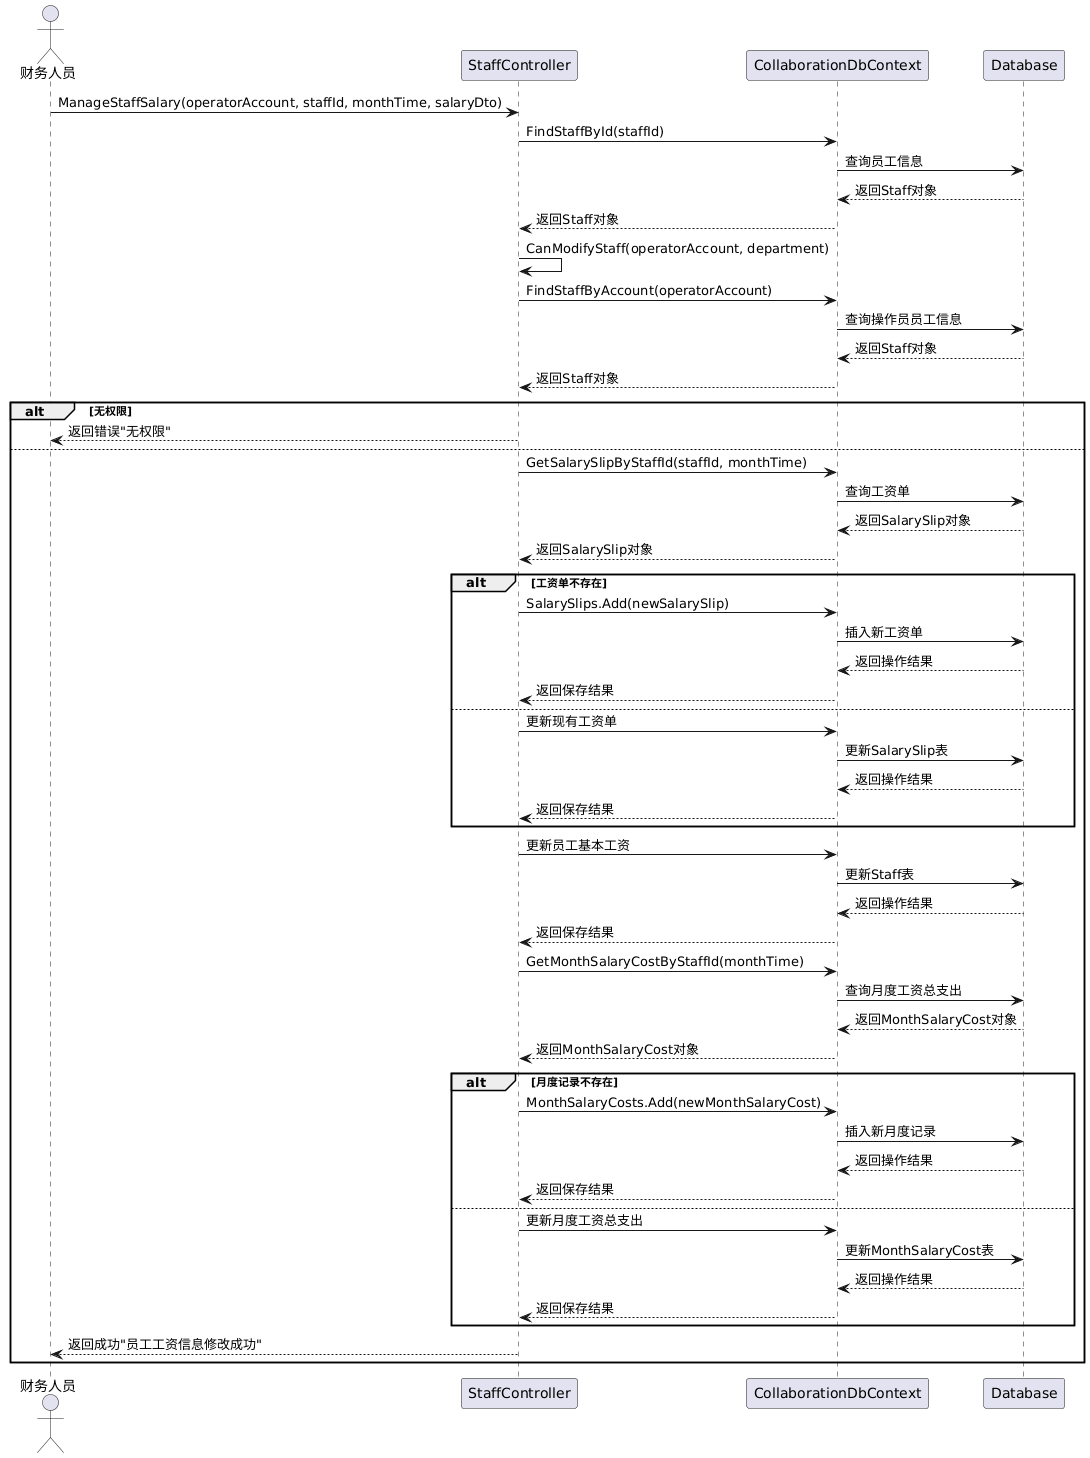
\includegraphics[width=6.32153in,height=8.45556in]{media/media/image18.png}

临时权限管理:

~ ~ ~ ~ {[}HttpPost("temporary\_authority"){]}

~ ~ ~ ~ public async Task\textless{}IActionResult\textgreater{}
ManageTemporaryAuthority(

~ ~ ~ ~ ~ ~ {[}FromQuery, Required{]} string operatorAccount,

~ ~ ~ ~ ~ ~ {[}FromBody, Required{]} TempAuthorityDto dto)

~ ~ ~ ~ {[}HttpDelete("revoke\_temporary\_authority"){]}

~ ~ ~ ~ public async Task\textless{}IActionResult\textgreater{}
RevokeTemporaryAuthority(

~ ~ ~ ~ ~ ~ {[}FromQuery, Required{]} string operatorAccount,

~ ~ ~ ~ ~ ~ {[}FromQuery, Required{]} string staffAccount,

~ ~ ~ ~ ~ ~ {[}FromQuery, Required{]} int eventId)

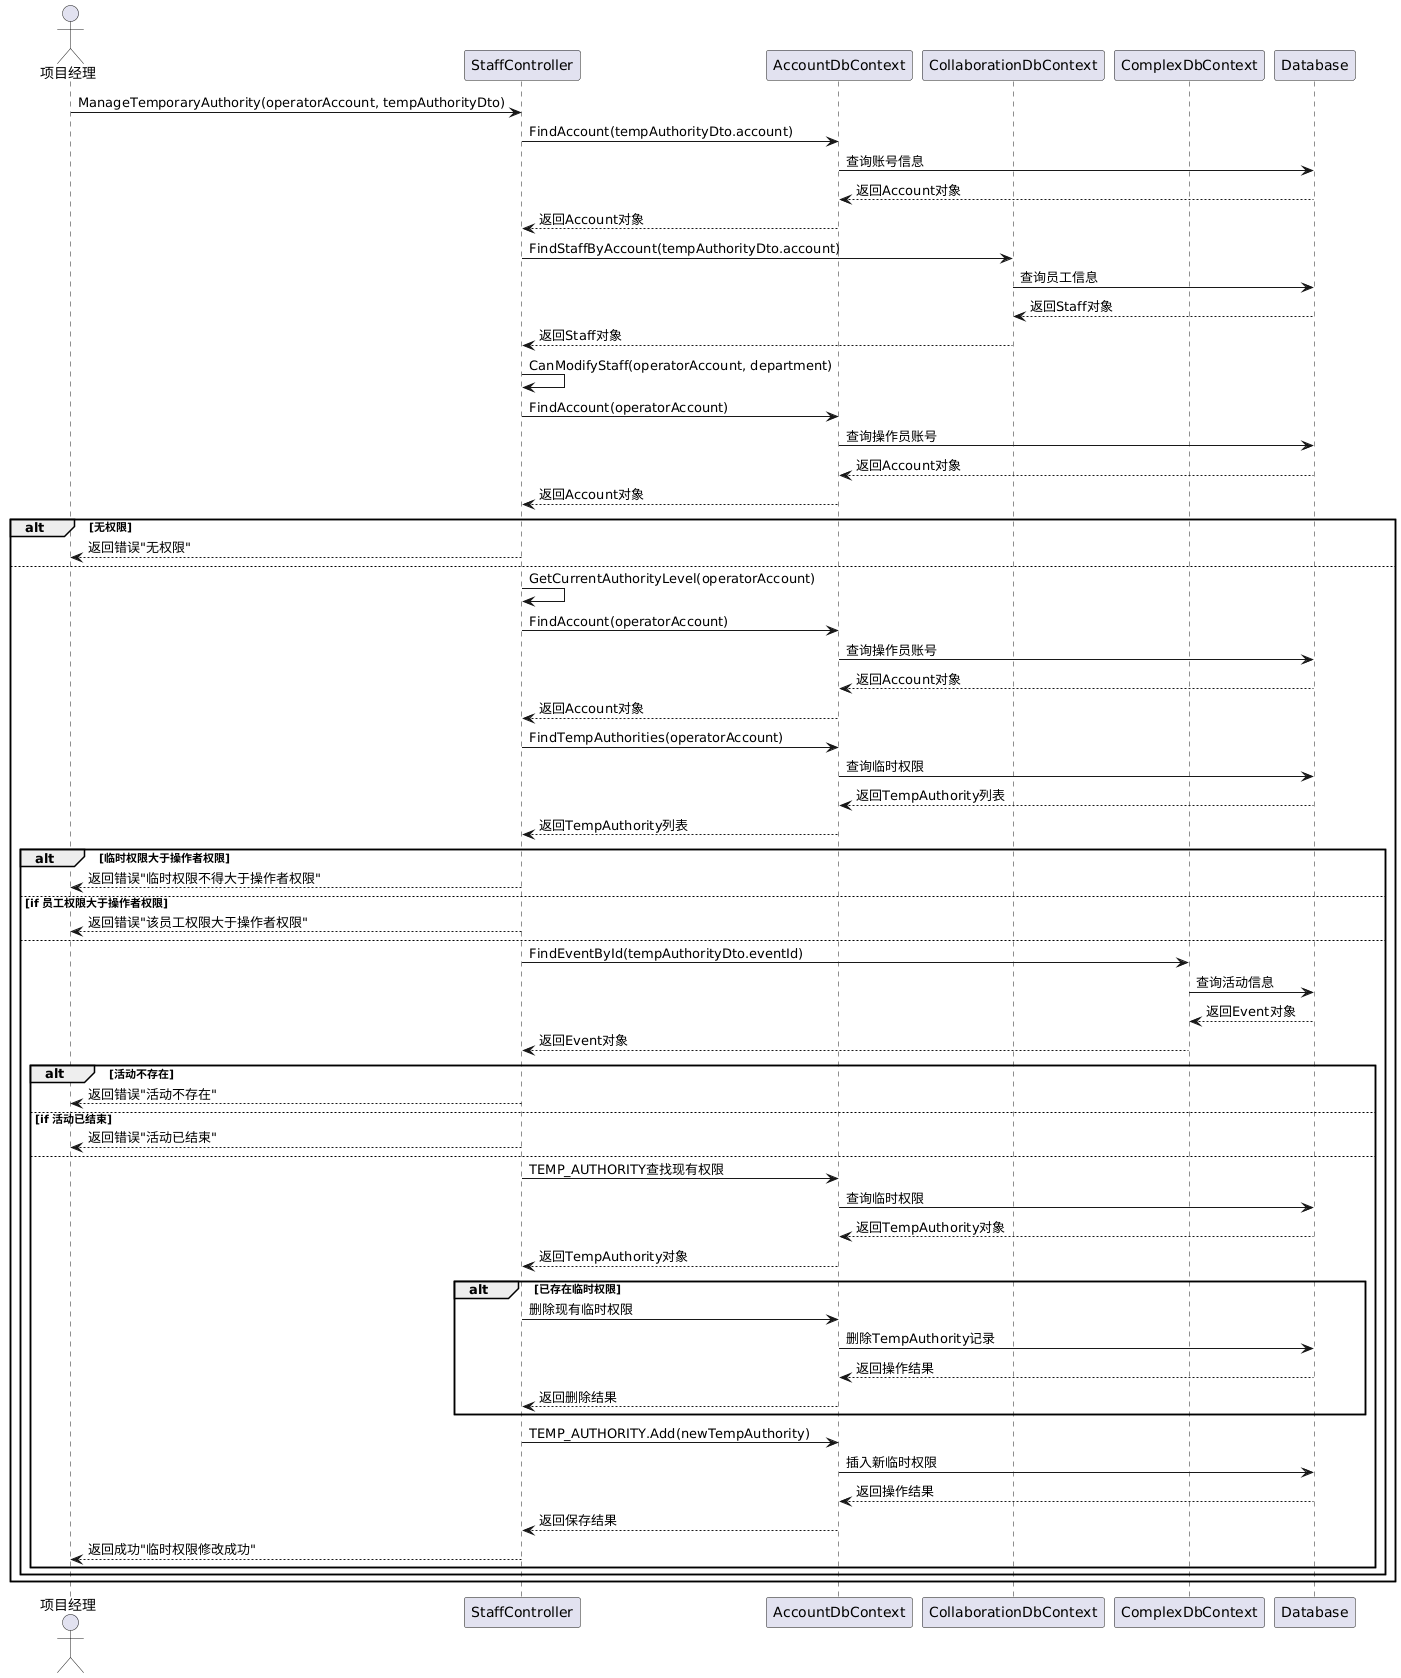
\includegraphics[width=6.28194in,height=7.52361in]{media/media/image19.png}

\hypertarget{ux6570ux636eux5e93ux8bbeux8ba1}{%
  \section{数据库设计}\label{ux6570ux636eux5e93ux8bbeux8ba1}}

数据库设计(E-R图,关系图,关系模式说明)

\begin{enumerate}
  \def\labelenumi{\Alph{enumi}.}
  \item
        \protect\hypertarget{_Toc153177886}{}{\protect\hypertarget{_Toc153186299}{}{\protect\hypertarget{_Toc155321769}{}{\protect\hypertarget{_Toc77076522}{}{}}}}图表索引
\end{enumerate}

\protect\hyperlink{_Toc394245023}{{图 2‑1 **功能实现} 2}

\protect\hyperlink{_Toc394245026}{{表格 2‑1 **功能的动作序列} 2}

\end{document}
